\documentclass{article}
\usepackage{geometry}
\usepackage{titling}
\usepackage{amsmath}
\usepackage{graphicx}
\usepackage{hyperref}

\hypersetup{colorlinks=true,urlcolor=cyan,linkcolor=blue}


\title{Longitudinal Study of RL and OHC-DC Vibrations}
\author{Brian Frost}
\date{March 28 2022}
\pretitle{\begin{center}\huge}
\posttitle{\end{center}}
\preauthor{\begin{center}\small}
\postauthor{\end{center}}
\predate{\begin{center}\footnotesize}
\postdate{\end{center}}
\setlength{\droptitle}{-40pt}

\begin{document}
\maketitle

\section{Introduction}

\par{In our MOH 2022 manuscript, we provided a method for aligning BM and OHC in longitudinal cross-sections and measuring these structures along the tonotopic axis. In Frost et al, 2022, we provide a single example of such a ``displacement-corrected" measurement of OHC and BM taken at 80 dB SPL. This example shows that single-measurement comparisons of OHC and BM can lead to a substantial mischaracterization of the relative phases of these two structures.}
\par{In this study, we observe displacement-corrected measurements of OHC and BM in single tonotopic cross-sections along a 160 $\mu$m longitudinal span in the base of the gerbil cochlea at 50, 65 and 80 dB SPL. We have taken care to measure both at the base of the OHCs near the Deiters' cells (OHC-DC) and at the apex of the OHCs (reticular lamina, RL). In doing so, we can extend our understanding of differences between RL and OHC-DC motion with respect to one another, and with respect to BM as well.}
\par{We have verified the longitudinal spread via our acquisition method (MOH 2022), our planar approximation method (Frost et al, 2022), as well as by observing the traveling wave phase. In our acquisition method, we attempted to achieve a 15um longitudinal step size. In verifying with our planar approximation method, we achieved a 16 $\mu$m step size which is remarkably close, validating the acquisition method.}
\par{Our measurements are taken at an angle $51^{\text{o}}$ from the BM normal, so they represent projections with significant components in both the longitudinal and transverse direction. We have taken care to ensure that there is no radial component to our measurements.}
\par{In this document, I will show several representative data sets. For a more complete exposition of the data from this experiment, see the larger data document from March 28.}

\section{OHC-DC Measurements}
\par{Run 9 included measurements at 11 positions spaced ~16 $\mu$m apart, ranging from the 26 kHz place to the 21.5 kHz place. Aligned OHC and BM lie about 3 measurement positions apart, so we were able to align 8 OHC-DC points with BM points in the same cross-section (a 128 $\mu$m longitudinal span). }
\subsection{Longitudinal traveling wave}
\par{First we verify that we are actually moving longitudinally by displaying BM phase at 80 dB (where SNR is best) as a function of frequency at all 11 positions. This can be seen in Fig. \ref{long}. The traveling wave phase shift can be seen nicely, with phase falling off faster at more apical locations (corresponding to higher position indeces).}

\begin{figure}
	\centering
	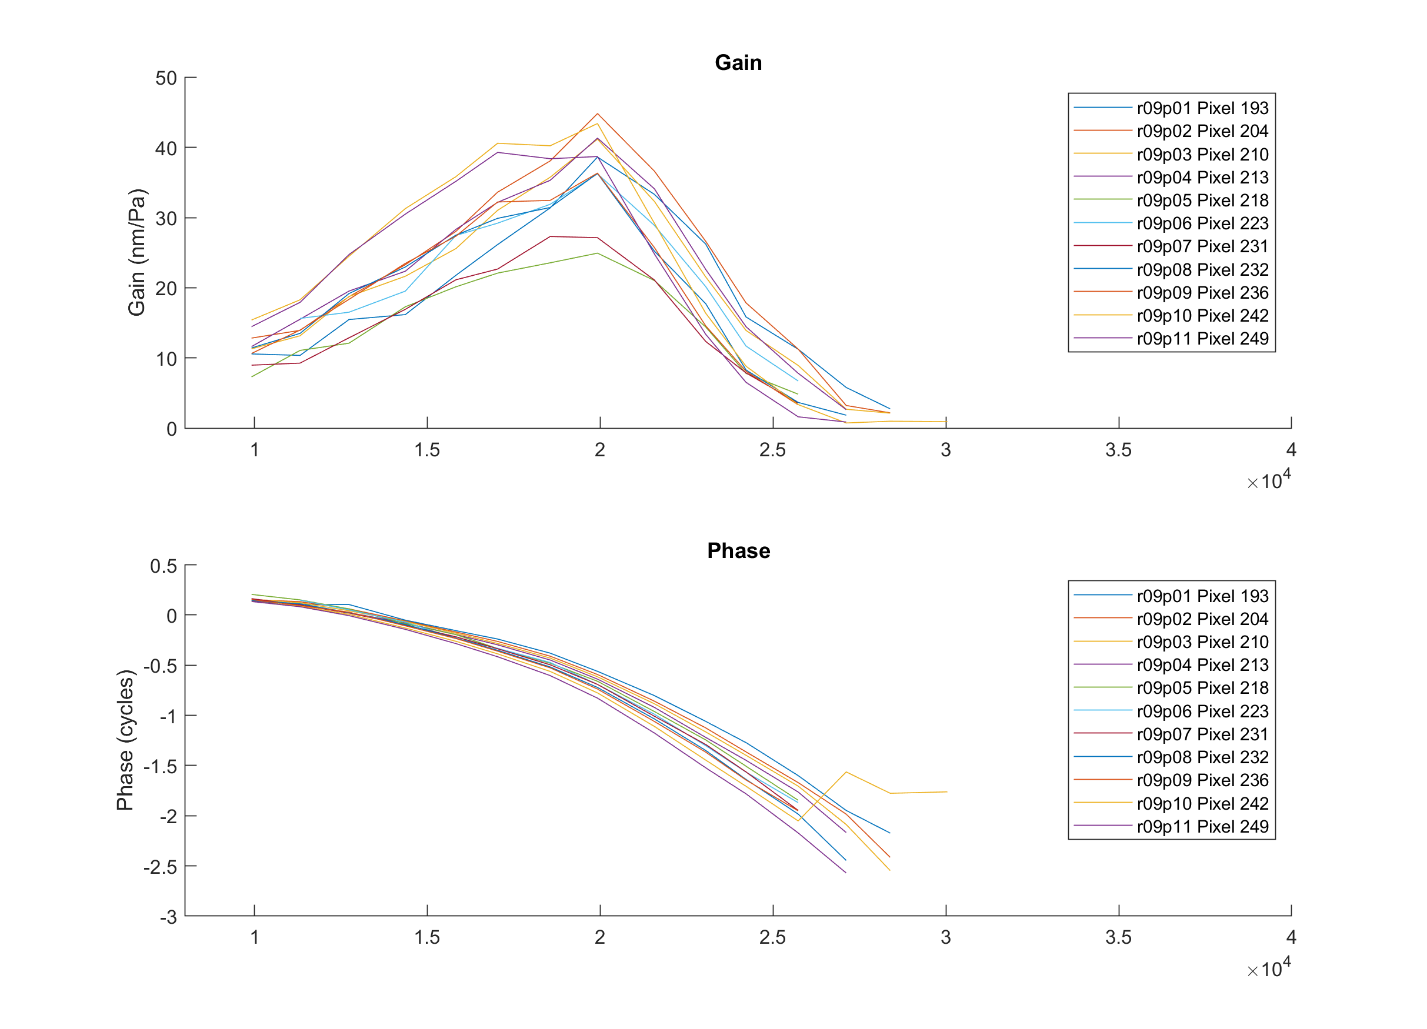
\includegraphics[width=.8\textwidth]{Figures/longshift.png}
	\caption{BM amplitudes and phases from run 9 at 80 dB, spaced 16 $\mu$m apart longitudinally. Increase in the position index corresponds to moving towards apex. The traveling wave shift is clear in the phase, wherein more apical phase responses fall off at lower frequencies than basal ones.}
	\label{long}
\end{figure}

\subsection{Single-measurement comparisons}
\par{First we look at OHC-DC and BM in a single measurement at 65 dB, uncorrected for longitudinal displacement. Consider Fig \ref{ohcdcp165db}, in which points at the BM and within the measured OHC region have been chosen to plot magnitude and phase. From the image, it seems clear that the first point chosen in the A-Scan (pixel 217) is right at the OHC base, whereas the other ones may be at the base of other OHCs in the same cross-section or may be closer to the middle of an OHC. This isn't particularly clear from the resolution of our system.}
\par{Observing the gain, all points in the OHC region look characteristically similar with gain significantly larger than BM across the bulk of the frequency range. The phase shows that OHC in all regions slightly lead BM at low frequencies, then around 0.8 BF start to lag. The lag increases as frequency increases, and accumulates faster for points further apical (deeper). This could have to do with traveling wave phase accumulation -- we need to observe aligned points to be sure!}
\par{These data presented at 65 dB SPL and at a single position are representative of what we see at all positions for 50 dB and 65 dB SPL.}

\begin{figure}
	\centering
	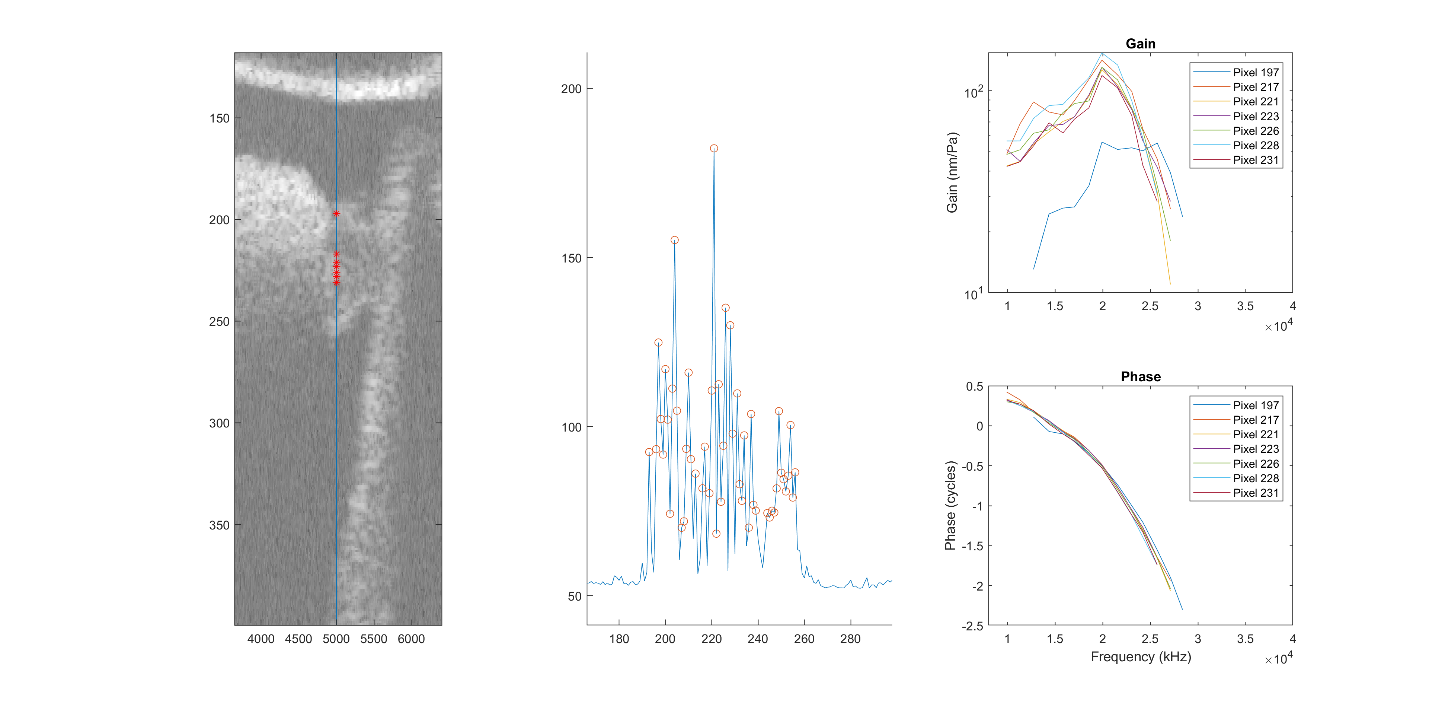
\includegraphics[width=\textwidth]{Figures/ohcdcp165dB.png}
	\caption{B-Scan containing an A-Scan along which a single measurement was taken at 65 dB SPL, zoomed-in averaged A-Scan magnitude along the marked axis, and magnitude and phase curves for the selected pixels. Points at the BM and within the OHC region are marked. As the angle of measurement is about 51 degrees, points lie more apical of one another as we move further down the A-Scan (down in the B-Scan, increasing pixel index, right in the A-Scan curve).}
	\label{ohcdcp165db}
\end{figure}

\par{The curves look different at 80 dB SPL -- consider Fig. \ref{ohcdcp1180db}, where we show two points in the OHC-DC region and a point on the BM. Here, OHC phase leads BM across frequency, only osculating BM phase around 0.8 BF. This difference is significant, and speaks to the difference between OHC-DC motion character at different SPLs.}
\par{These data at position 11 are representative of what we see at all positions for the 80 dB SPL stimulus.}

\begin{figure}
	\centering
	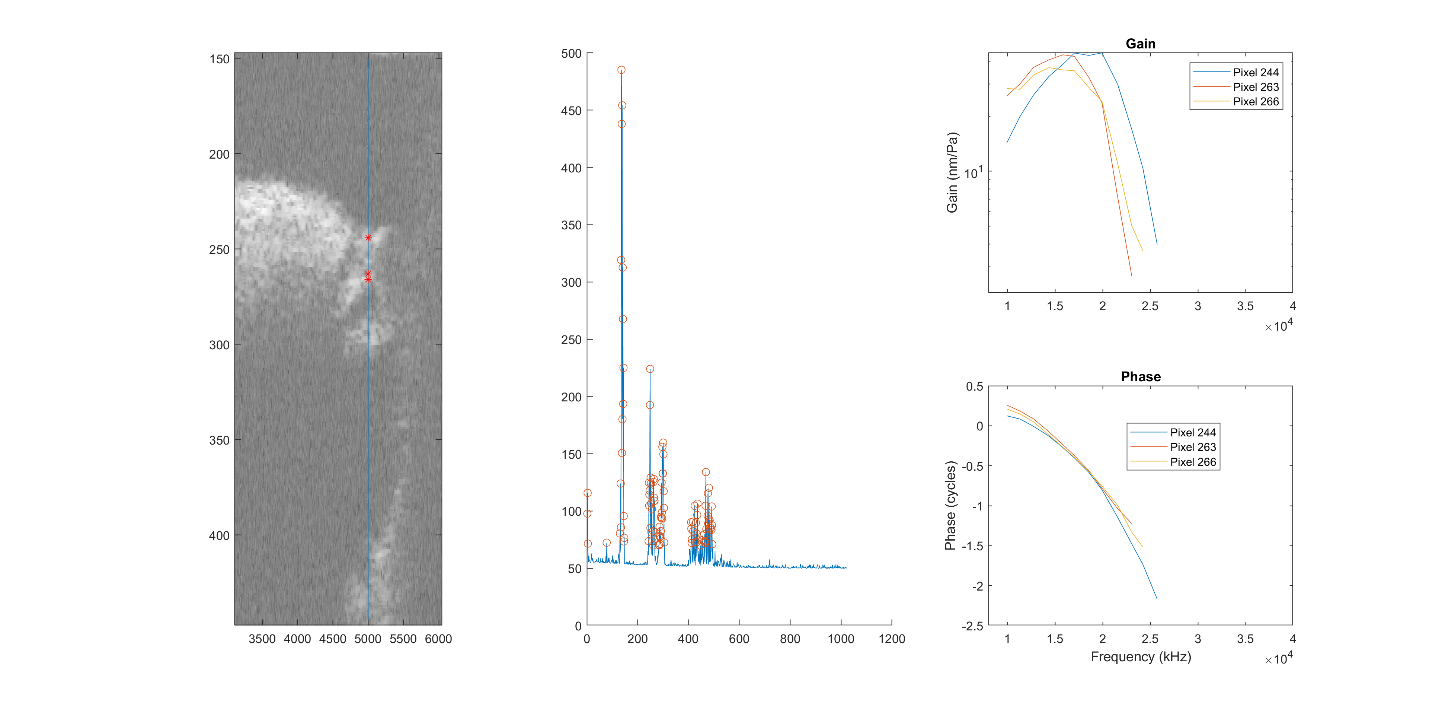
\includegraphics[width=\textwidth]{Figures/ohcdcp1180dB.png}
	\caption{B-Scan containing an A-Scan along which a single measurement was taken at 80 dB SPL, averaged A-Scan magnitude along the marked axis, and magnitude and phase curves for the selected pixels. Points at the BM and within the OHC region are marked. As the angle of measurement is about 51 degrees, points lie more apical of one another as we move further down the A-Scan (down in the B-Scan, increasing pixel index, right in the A-Scan curve).}
	\label{ohcdcp1180db}
\end{figure}

\subsection{Aligned BM and OHC-DC}
\par{More instructive are the OHC-DC and BM motions in the same anatomical cross-section. Figs. \ref{2pt50}, \ref{2pt65} and \ref{2pt80} show the gain and phase of BM and two points along the OHC region -- one deeper into the A-Scan than the other -- at 50, 65 and 80 dB SPL respectively. While at one measurement location the different OHC points along the A-Scan appear to move differently, correcting for longitudinal displacement shows that their phases are more-or-less exactly the same. This suggests that we are measuring several points at the base of different OHCs, rather than points further towards the apex of the OHC.}
\par{Across frequency, OHC-DC phase at this angle seems to lead BM phase. At 80 dB SPL, the lead is smallest around 0.8 BF, and is largest at very low and very high frequencies. This is consistent with what is presented in Frost et al, 2022. We also see that the OHC phase starts to flatline at high frequencies, potentially corresponding to a takeover of the fast wave. The OHC phase slope changes here, be more flat as well. This is consistent with a fast wave takeover.}
\par{At first glance, at 50 and 65 dB SPL our data look similar. However, the lead is more constant across frequency. This could be in part due to the fact that we do not have much high-frequency data. Also worth noting is that at 80 dB SPL, the OHC magnitude begins to fall off rapidly at a lower frequency than at lower SPL.}

\begin{figure}
	\centering
	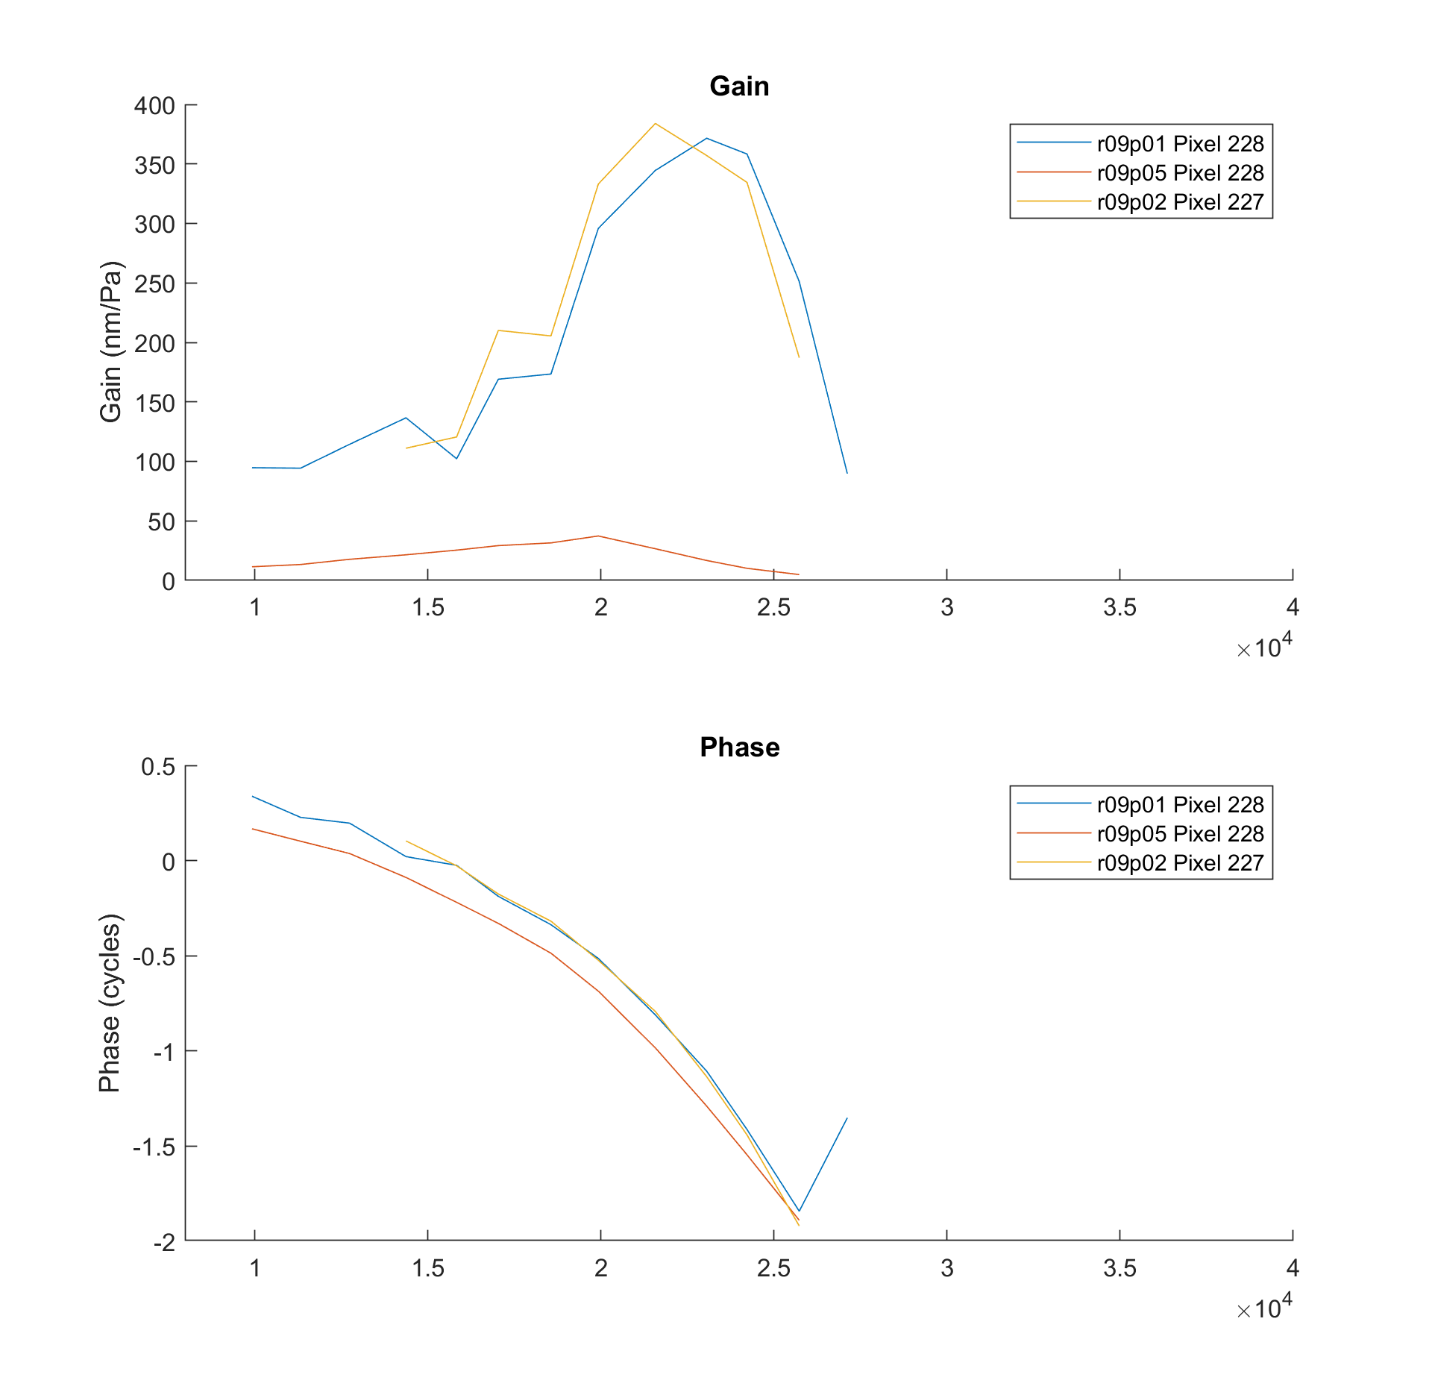
\includegraphics[width=\textwidth]{Figures/ohcdcp2pts50dB.png}
	\caption{Gain and phase at two points in the OHC-DC region with aligned BM. Blue: OHC position further from BM; Yellow: OHC position nearer to BM; Red: BM. Data taken at 50 dB SPL.}
	\label{2pt50}
\end{figure}

\begin{figure}
	\centering
	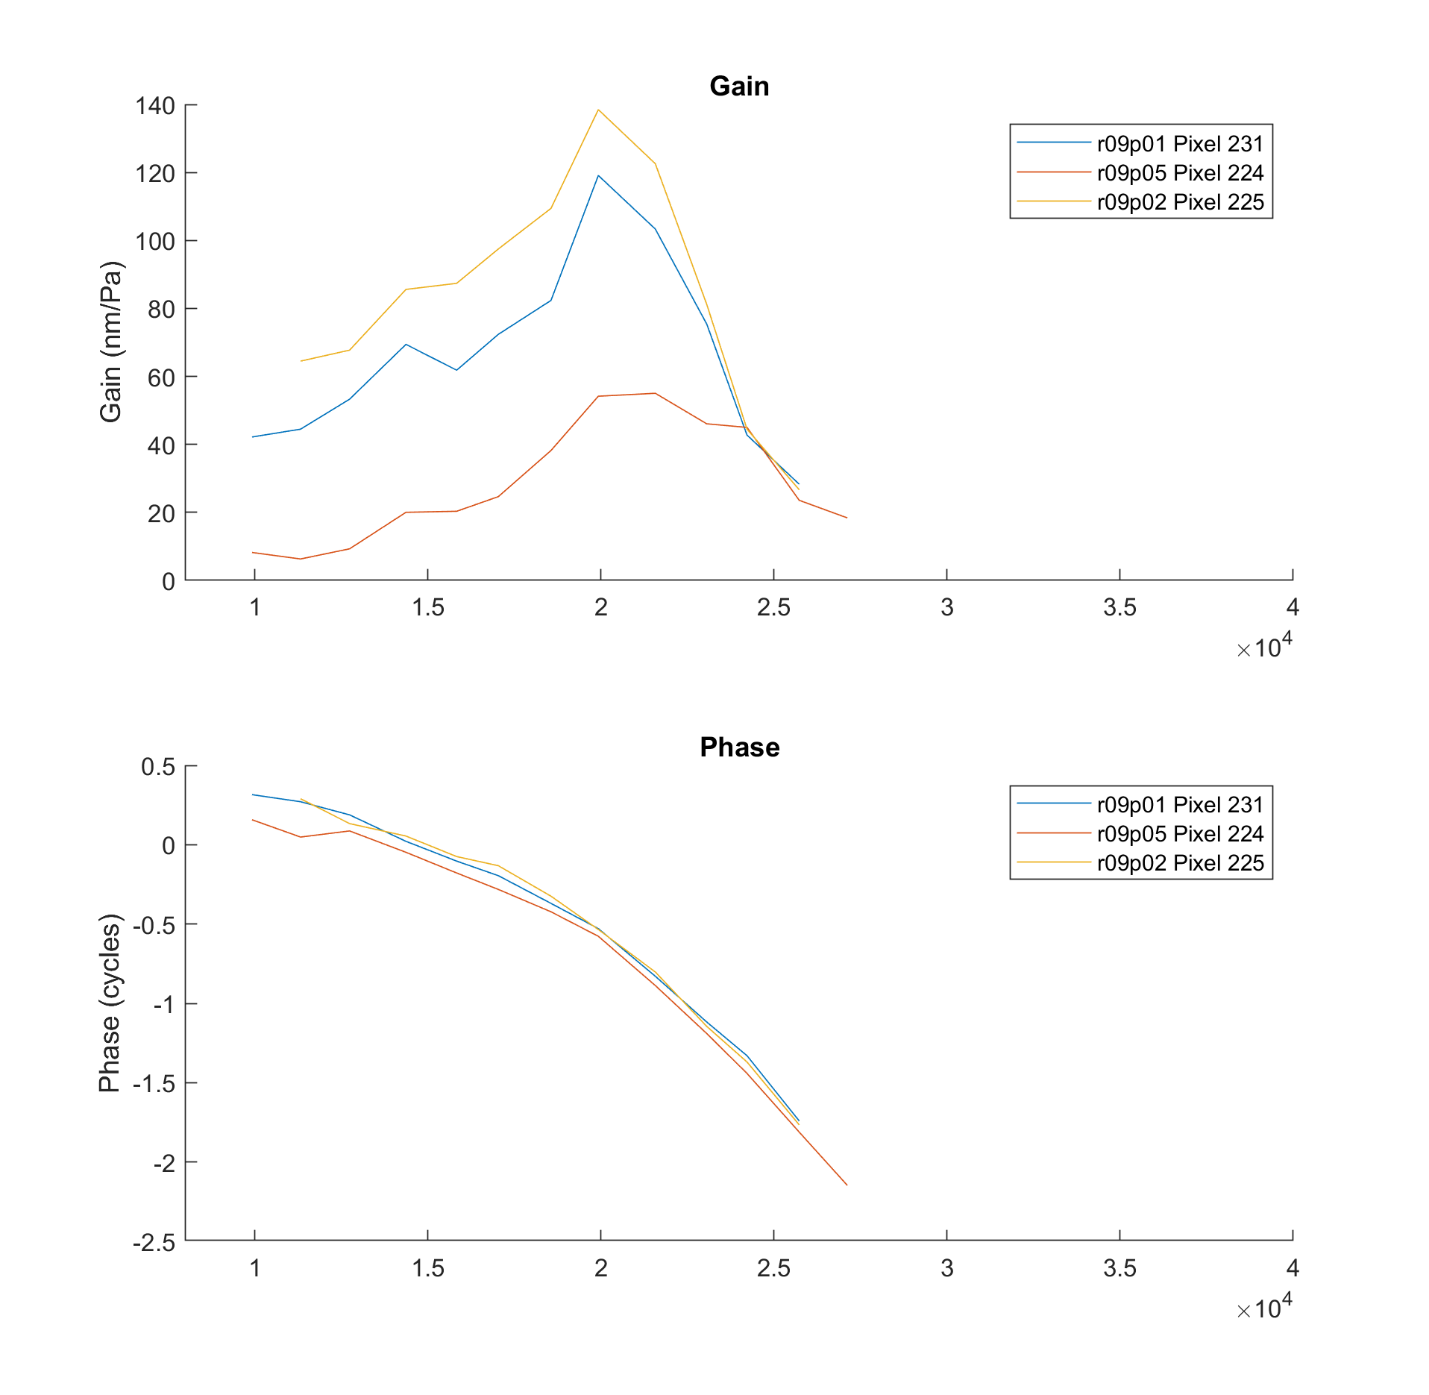
\includegraphics[width=\textwidth]{Figures/ohcdcp2pts65dB.png}
	\caption{Gain and phase at two points in the OHC-DC region with aligned BM. Blue: OHC position further from BM; Yellow: OHC position nearer to BM; Red: BM. Data taken at 65 dB SPL.}
	\label{2pt65}
\end{figure}

\begin{figure}
	\centering
	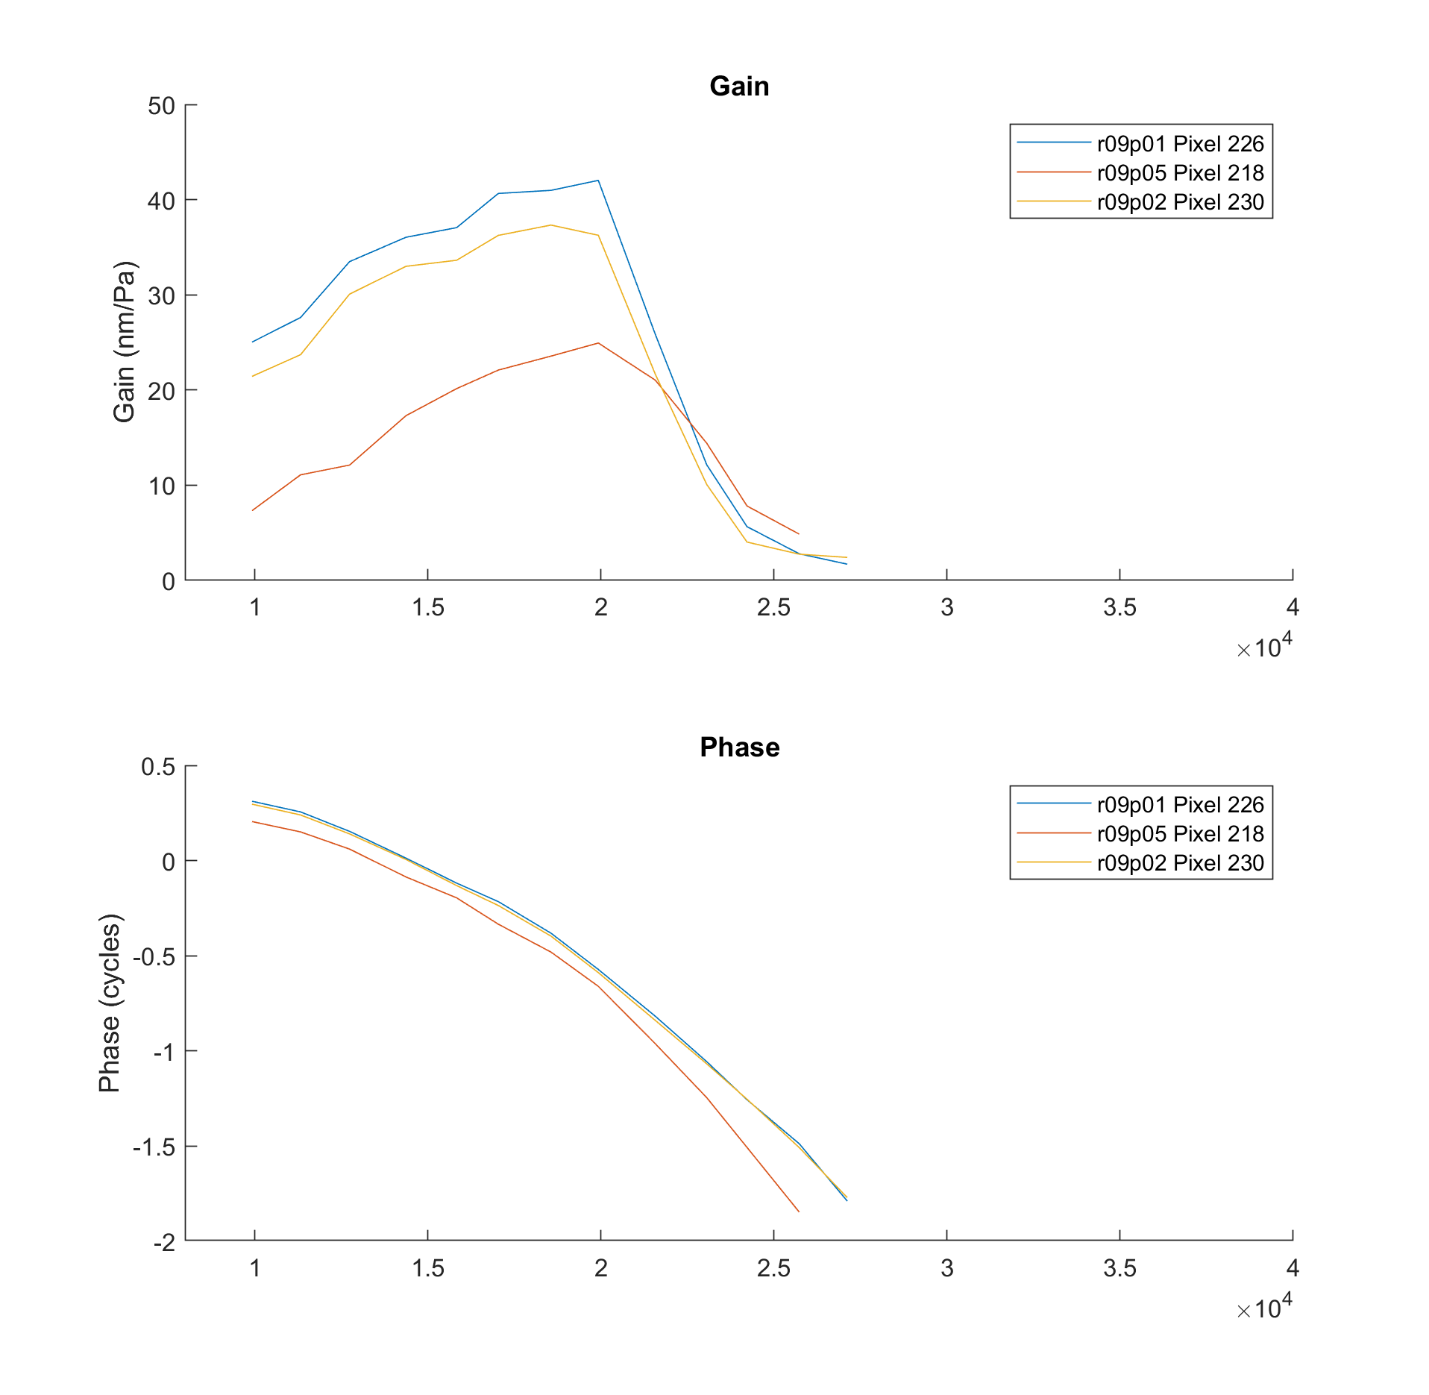
\includegraphics[width=\textwidth]{Figures/ohcdcp2pts80dB.png}
	\caption{Gain and phase at two points in the OHC-DC region with aligned BM. Blue: OHC position further from BM; Yellow: OHC position nearer to BM; Red: BM. Data taken at 80 dB SPL.}
	\label{2pt80}
\end{figure}

\par{To gain more intuition, we look also at the OHC-DC phase re BM phase. This is shown in Figs \ref{ohcdcbm50}, \ref{ohcdcbm65} and \ref{ohcdcbm80} for 50, 65 and 80 dB SPL. We display the phase difference for all aligned pairs as well as the average. Our data at 50 dB SPL is very poor, but where we have data we see an average lead on the orfer of 0.08 cycles, or ~30 degrees. At 65 dB SPL our data is better. The lead seems to decrease slowly and monotonically from as high as 0.2 cycles (~72 degrees) to a more constant lead of around 0.05 cycles (~20 degrees). At high frequencies, we see similar behavior to our 50 dB data. At low frequencies, we did not have 50 dB data so we cannot make any comparisons.}
\par{At 80 dB SPL, much like at 65 dB SPL, we see a large low-frequency lead on the order of 70 degrees. It decreases near the BF region, just like at 50 and 65 dB SPL. Then, at high frequencies, it increases rapidly. Comparing to the data above, this rapid increase in lag occurs around where the OHC magnitude flattens out, corresponding potentially to a takeover of the fast wave. Interestingly, the OHC dropoff in magnitude occurs at a much lower frequency than BM at this SPL, and so too does the fast wave takeover. This is why we see a larger high-frequency lead at 80 dB SPL than at lower SPL.}

\begin{figure}
	\centering
	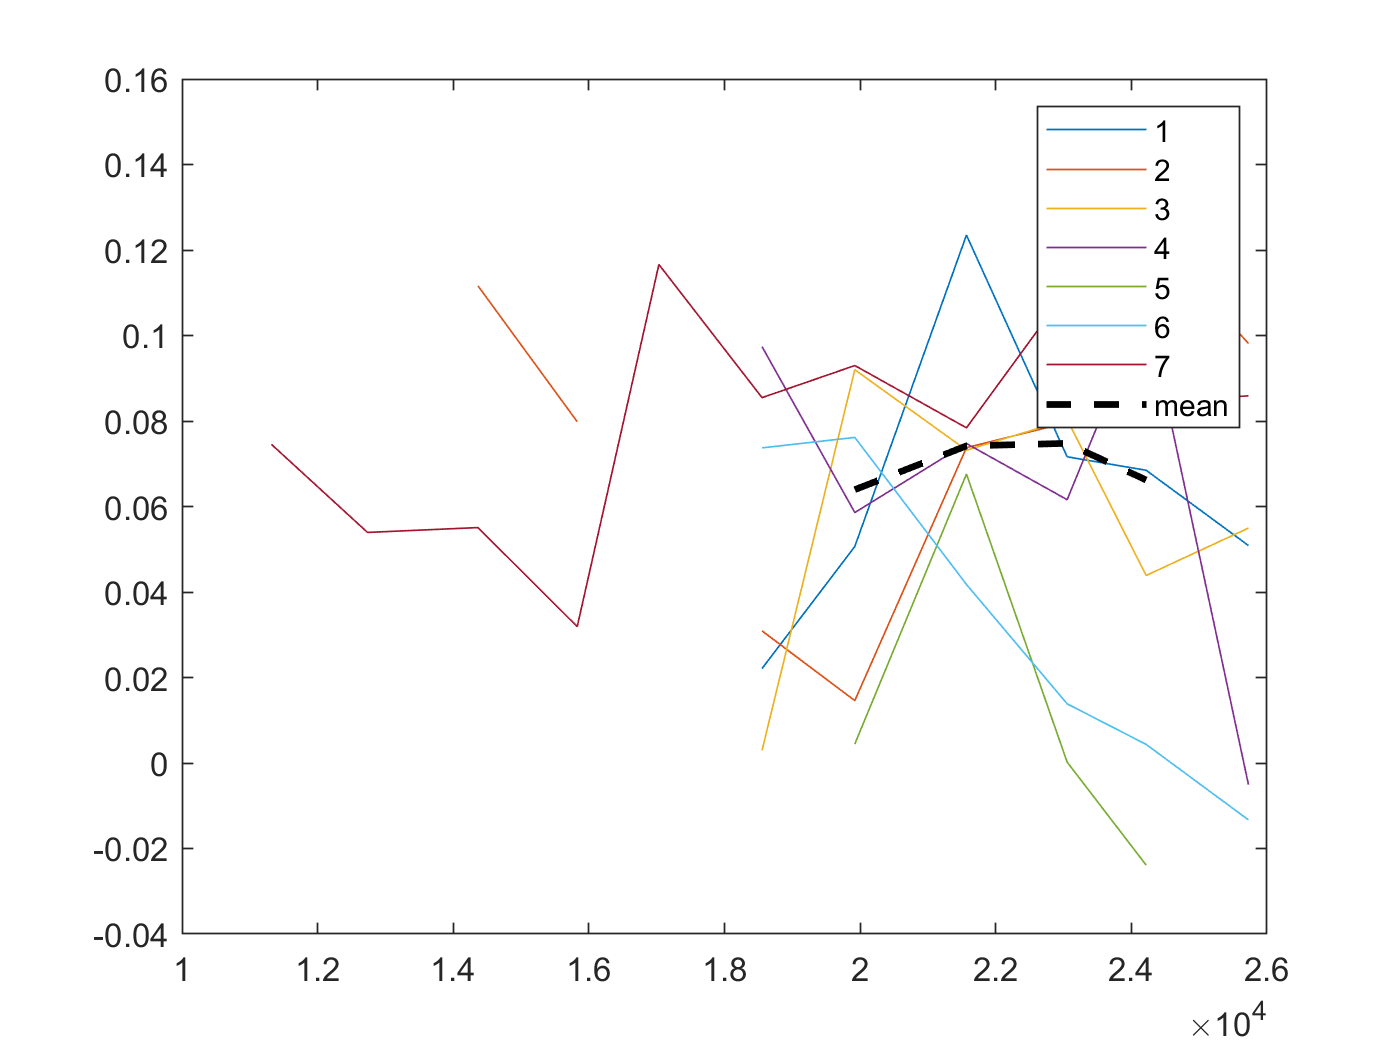
\includegraphics[width=.7\textwidth]{Figures/ohcdcbm50.png}
	\caption{OHC phase re aligned BM at 7 positions, with arithmetic mean. 50 dB SPL.}
	\label{ohcdcbm50}
\end{figure}

\begin{figure}
	\centering
	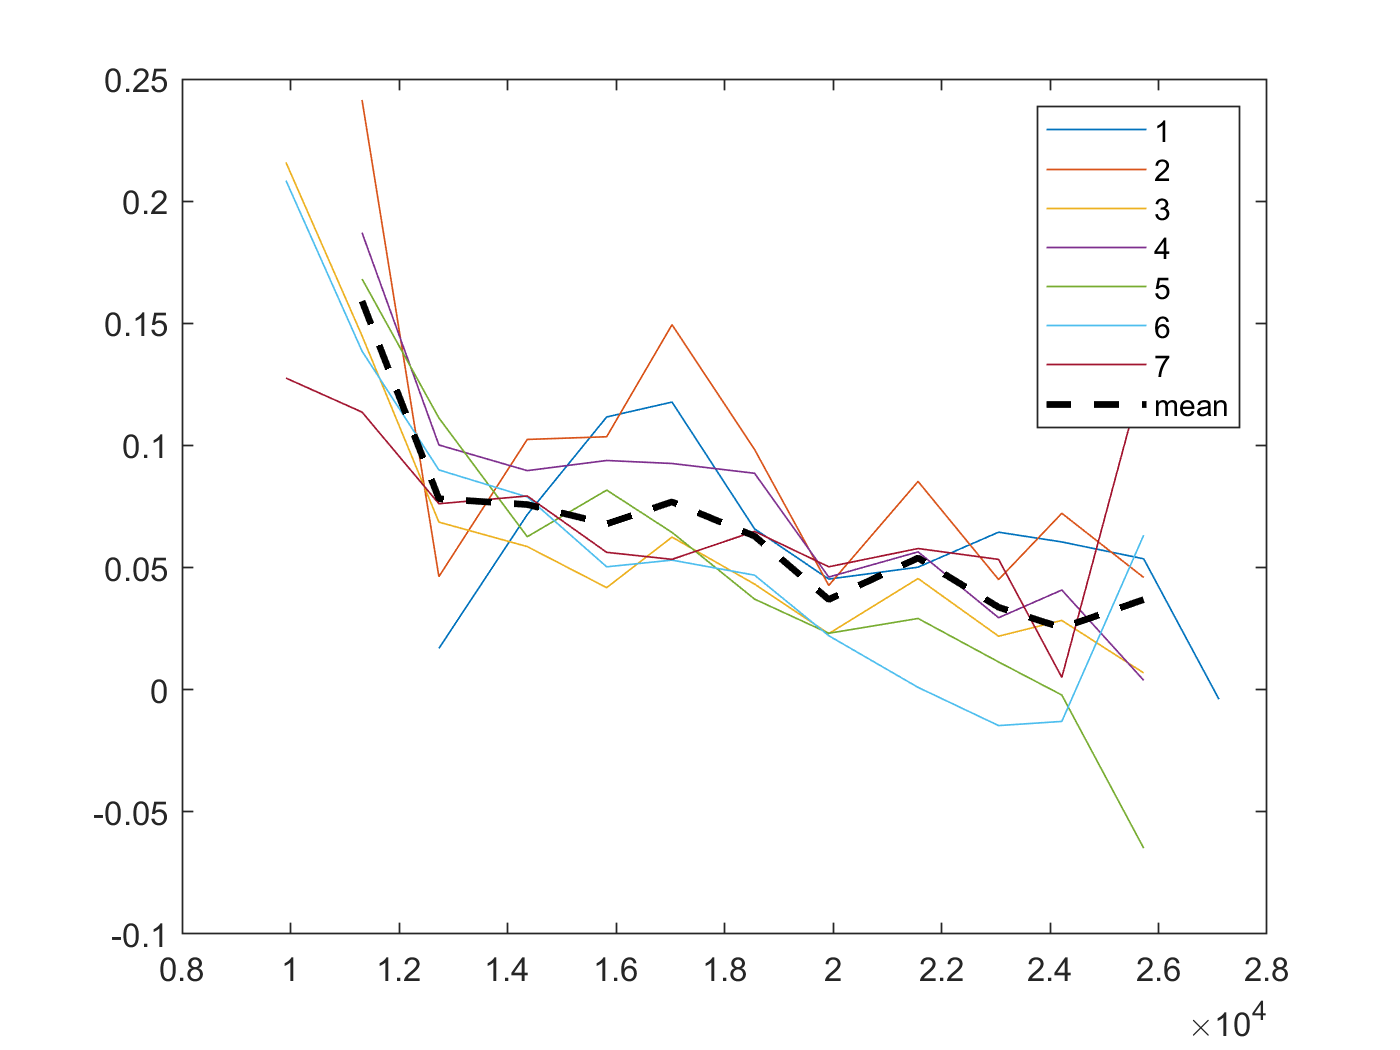
\includegraphics[width=.7\textwidth]{Figures/ohcdcbm65.png}
	\caption{OHC phase re aligned BM at 7 positions, with arithmetic mean. 65 dB SPL.}
	\label{ohcdcbm65}
\end{figure}

\begin{figure}
	\centering
	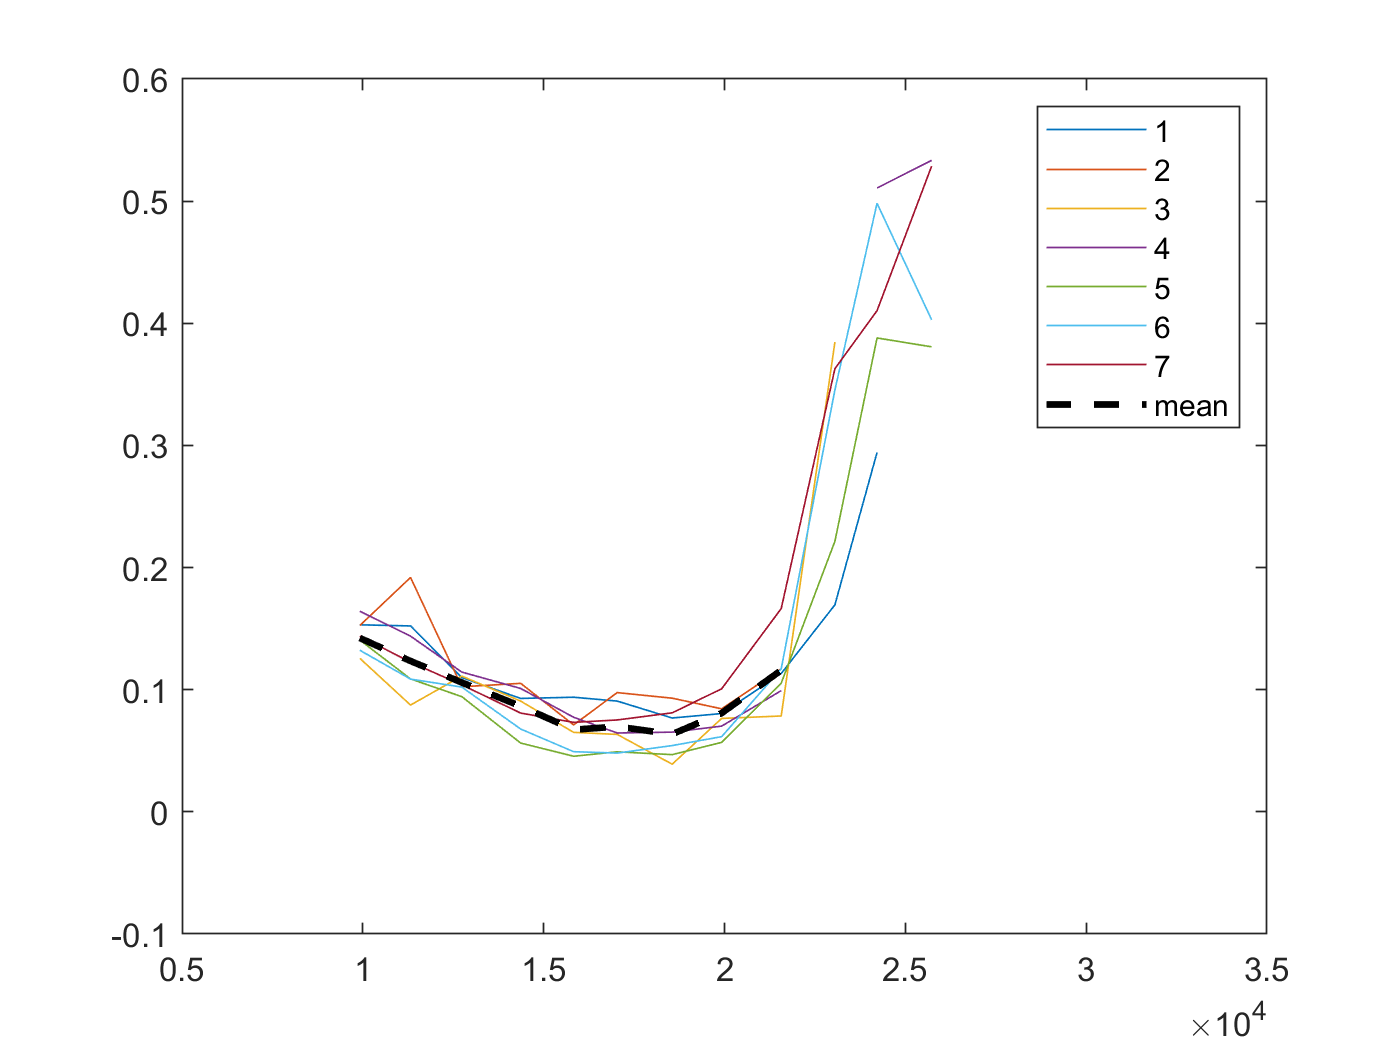
\includegraphics[width=.7\textwidth]{Figures/ohcdcbm80.png}
	\caption{OHC phase re aligned BM at 7 positions, with arithmetic mean. 80 dB SPL.}
	\label{ohcdcbm80}
\end{figure}

\par{From these figures, one may get the idea that there is little difference in the phase as a function of SPL. This is not quite true. Observing the OHC phase at three SPLs at a single position, as in Fig. \ref{ohcdcspls}, shows that at low frequencies lower SPL leads higher SPL, and at high frequencies high SPL leads low SPL. Very interestingly, the phases all seem to cross at ~BF. The data is consistent in this sense at all tested locations.}

\begin{figure}
	\centering
	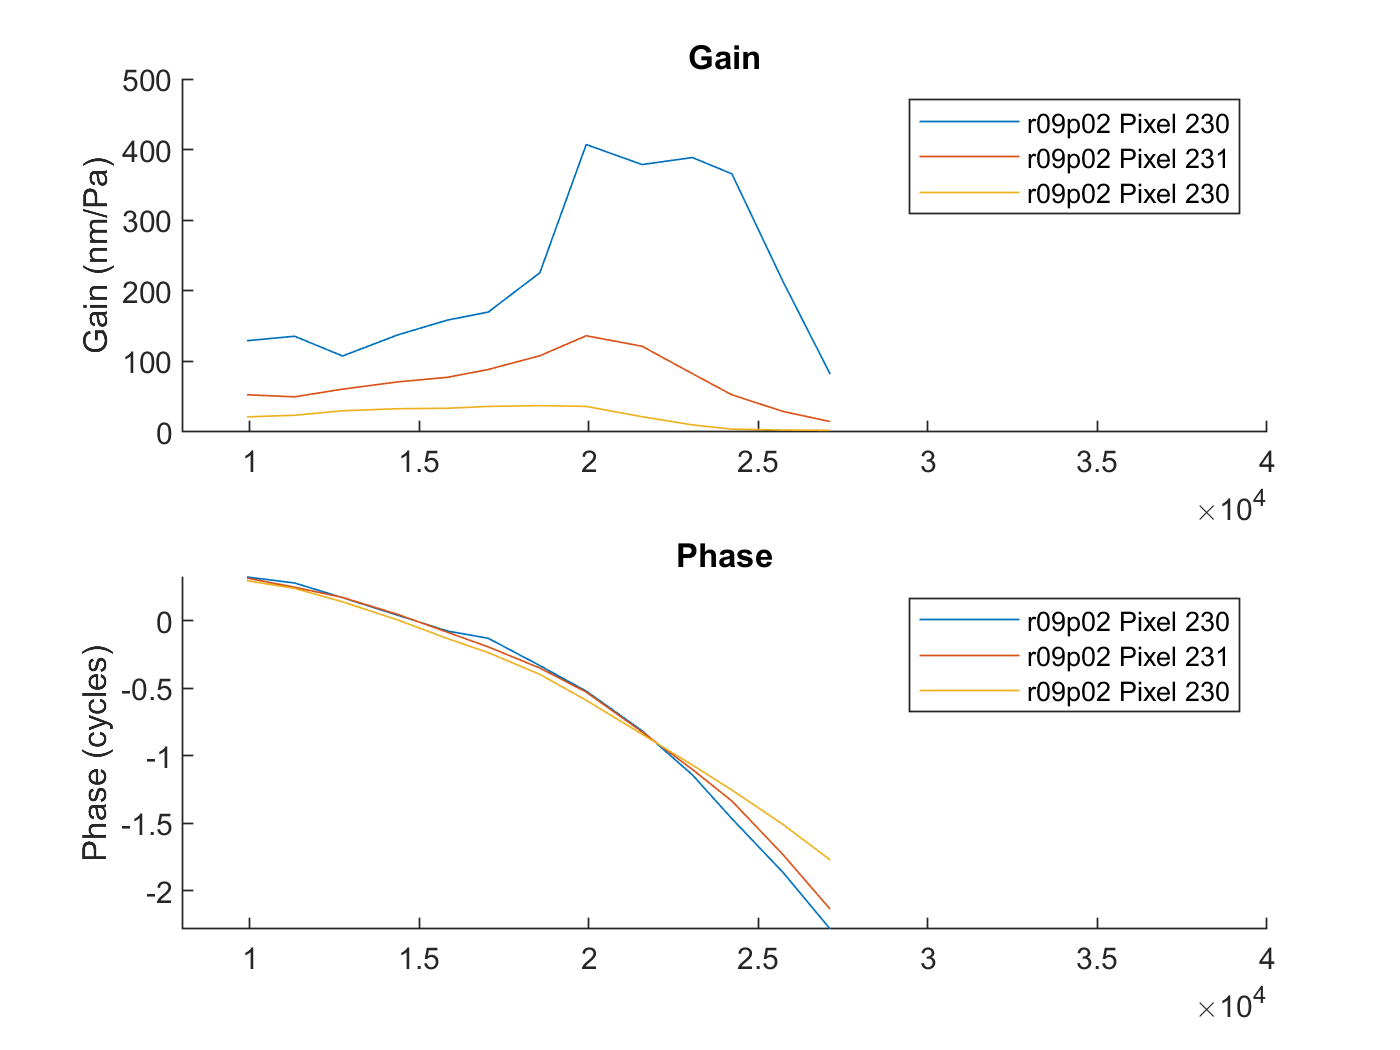
\includegraphics[width=.7\textwidth]{Figures/ohcdcspls.png}
	\caption{OHC-DC gain and phase at one position across SPLs. Blue: 50 dB; Red: 65 dB; Yellow: 80 dB.}
	\label{ohcdcspls}
\end{figure}

\subsection{Preliminary theories for why we see these motion patterns}
\par{We reconstructed some OHC motions at 80 dB SPL in Frost MOH 2022, and saw that the lead across frequency was largely due to a longitudinal component leading transverse OHC by ~half a cycle. The size of this contribution at 80 dB should depend only on the angle of measurement, which is a bit more longitudinal than transverse here. We see these same results here.}

\par{I am inclined to believe that the longitudinal displacements will be quite similar at all SPL in character (not magnitude), as they are likely caused by fluid motion. Assuming this is the cause of the lead at all SPL, the lead being lower supra-BF at 50 and 65 dB SPL means transverse OHC motion is probably more dominant there, and less dominant sub-BF. Interestingly at all SPL, they seem to be totally in phase at the BF. What this could correspond to is both a decrease in the longitudinal re transverse lead near BF (seen in the reconstructions!) and an increase in the transverse re longitudinal gain (seen in the reconstructions!). This would mean transverse OHC motion is dominant at BF and similar at all SPL in phase. This is just a hypothesis, that of course must be tested more rigorously.}


\section{RL Measurements}
\subsection{Aligned RL and BM measurements}
\par{Run 13 included measurements at 11 positions spaced ~16 $\mu$m apart, ranging from the 26 kHz place to the 21.5 kHz place. Our measurement angle is ~51 degrees from the normal to the BM. Aligned OHC and BM lie about 4 measurement positions apart, so we were able to align 7 RL points with BM points in the same cross-section (a 112 $\mu$m longitudinal span).}
\par{In Figs \ref{rlbm50}, \ref{rlbm65} and \ref{rlbm80} we show aligned RL and BM data at 50, 65 and 80 dB SPL respectively. At most points at 50 and 65 dB we see almost no difference between RL and BM. However, where we do see a difference, it is a high-frequency lead of BM re RL. This is similar to what we see in Ren’s data across SPL at high frequencies. However at low frequencies it is different – Ren sees a lead of RL re BM at low frequencies whereas we are seeing no difference.}
\par{At 80 dB, however, we see a strange change at all positions: an across-frequency lead of RL re BM in the form of a big jump. This is very similar to what we see in correcting the OHC-DC region for displacement.}

\begin{figure}
	\centering
	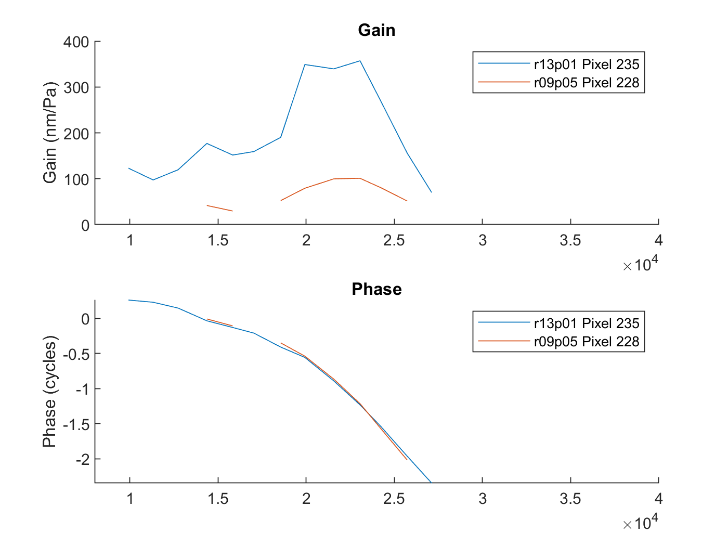
\includegraphics[width=.7\textwidth]{Figures/rlbm50.png}
	\caption{Gain and phase of aligned BM (red) and RL (blue) at 50 dB SPL.}
	\label{rlbm50}
\end{figure}

\begin{figure}
	\centering
	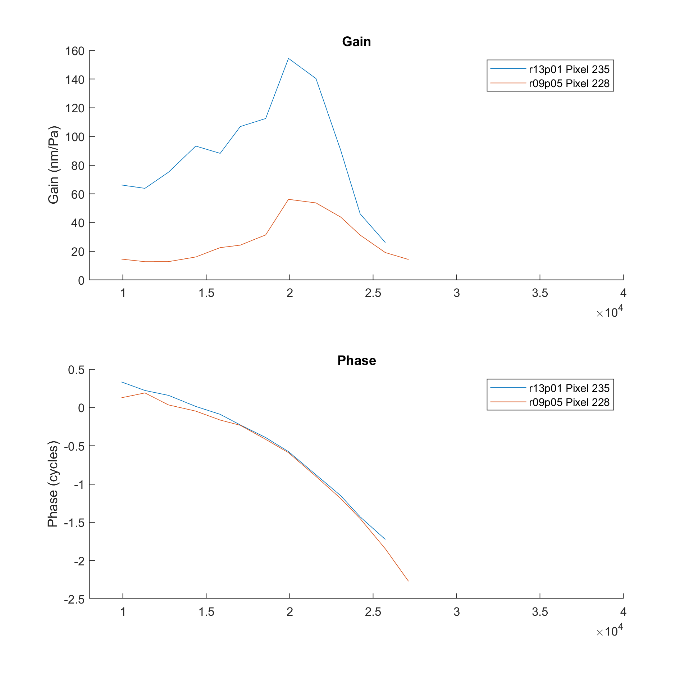
\includegraphics[width=.7\textwidth]{Figures/rlbm65.png}
	\caption{Gain and phase of aligned BM (red) and RL (blue) at 65 dB SPL.}
	\label{rlbm65}
\end{figure}

\begin{figure}
	\centering
	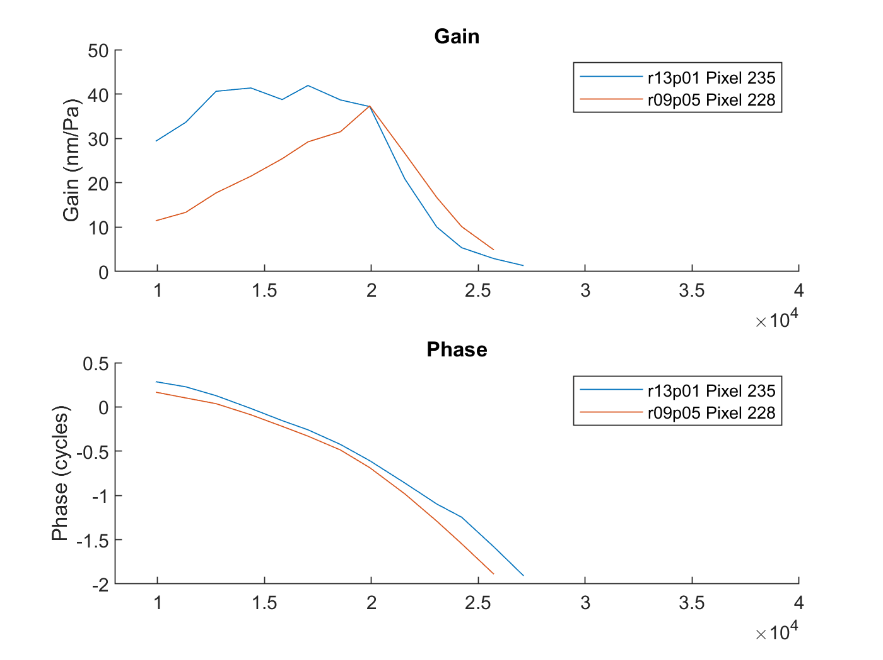
\includegraphics[width=.7\textwidth]{Figures/rlbm80.png}
	\caption{Gain and phase of aligned BM (red) and RL (blue) at 80 dB SPL.}
	\label{rlbm80}
\end{figure}

\subsection{Aligned RL and OHC-DC measurements}
\par{One of the most interesting comparisons to make is OHC-DC vs RL at this angle in the same cross-section. Dewey sees that OHC-DC and RL displacements are almost always out of phase by ~.5 cycles across frequency and SPL, with the difference decreasing slightly as SPL increases and near BF. We align OHC-DC and RL measurements and plot the two phases with one another at 50, 65 and 80 dB SPL in Figs \ref{rldc50}, \ref{rldc65} and \ref{rldc80} respectively. We also plot the differences and their averages in Figs \ref{rlredc50}, \ref{rlredc65} and \ref{rlredc80}. We should be careful to consider the effect the angle might have here.}

\begin{figure}
	\centering
	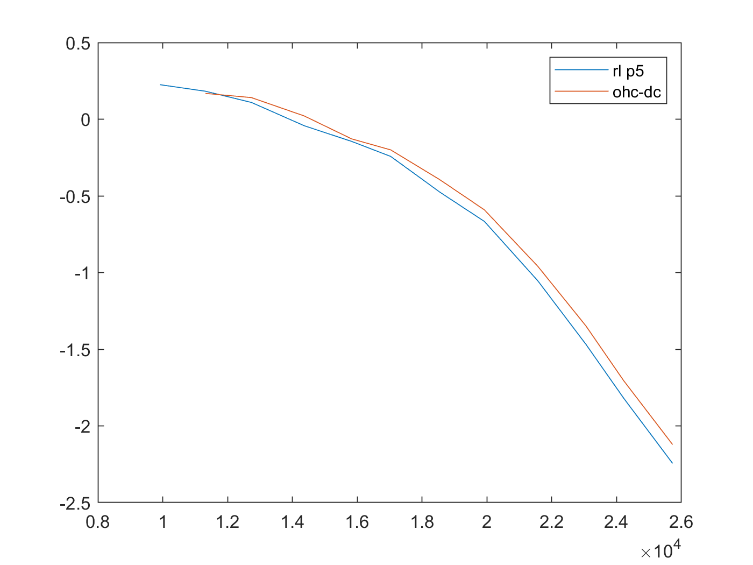
\includegraphics[width=.7\textwidth]{Figures/rldc50.png}
	\caption{Aligned RL (blue) and OHC-DC (red) phase responses at 50 dB SPL.}
	\label{rldc50}
\end{figure}

\begin{figure}
	\centering
	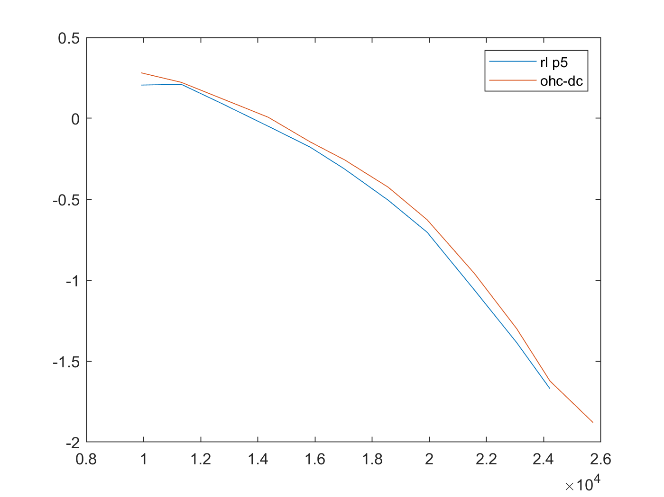
\includegraphics[width=.7\textwidth]{Figures/rldc65.png}
	\caption{Aligned RL (blue) and OHC-DC (red) phase responses at 65 dB SPL.}
	\label{rldc65}
\end{figure}

\begin{figure}
	\centering
	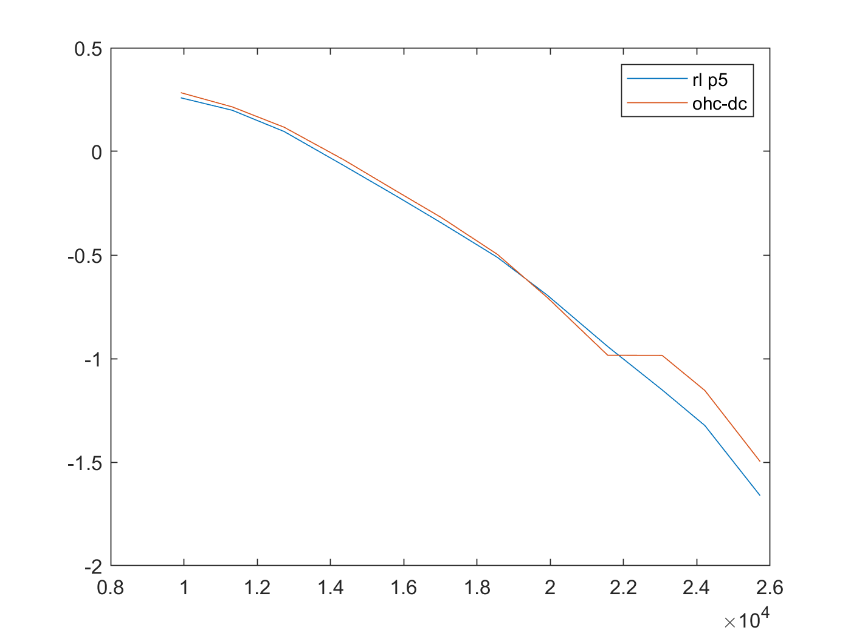
\includegraphics[width=.7\textwidth]{Figures/rldc80.png}
	\caption{Aligned RL (blue) and OHC-DC (red) phase responses at 80 dB SPL.}
	\label{rldc80}
\end{figure}

\begin{figure}
	\centering
	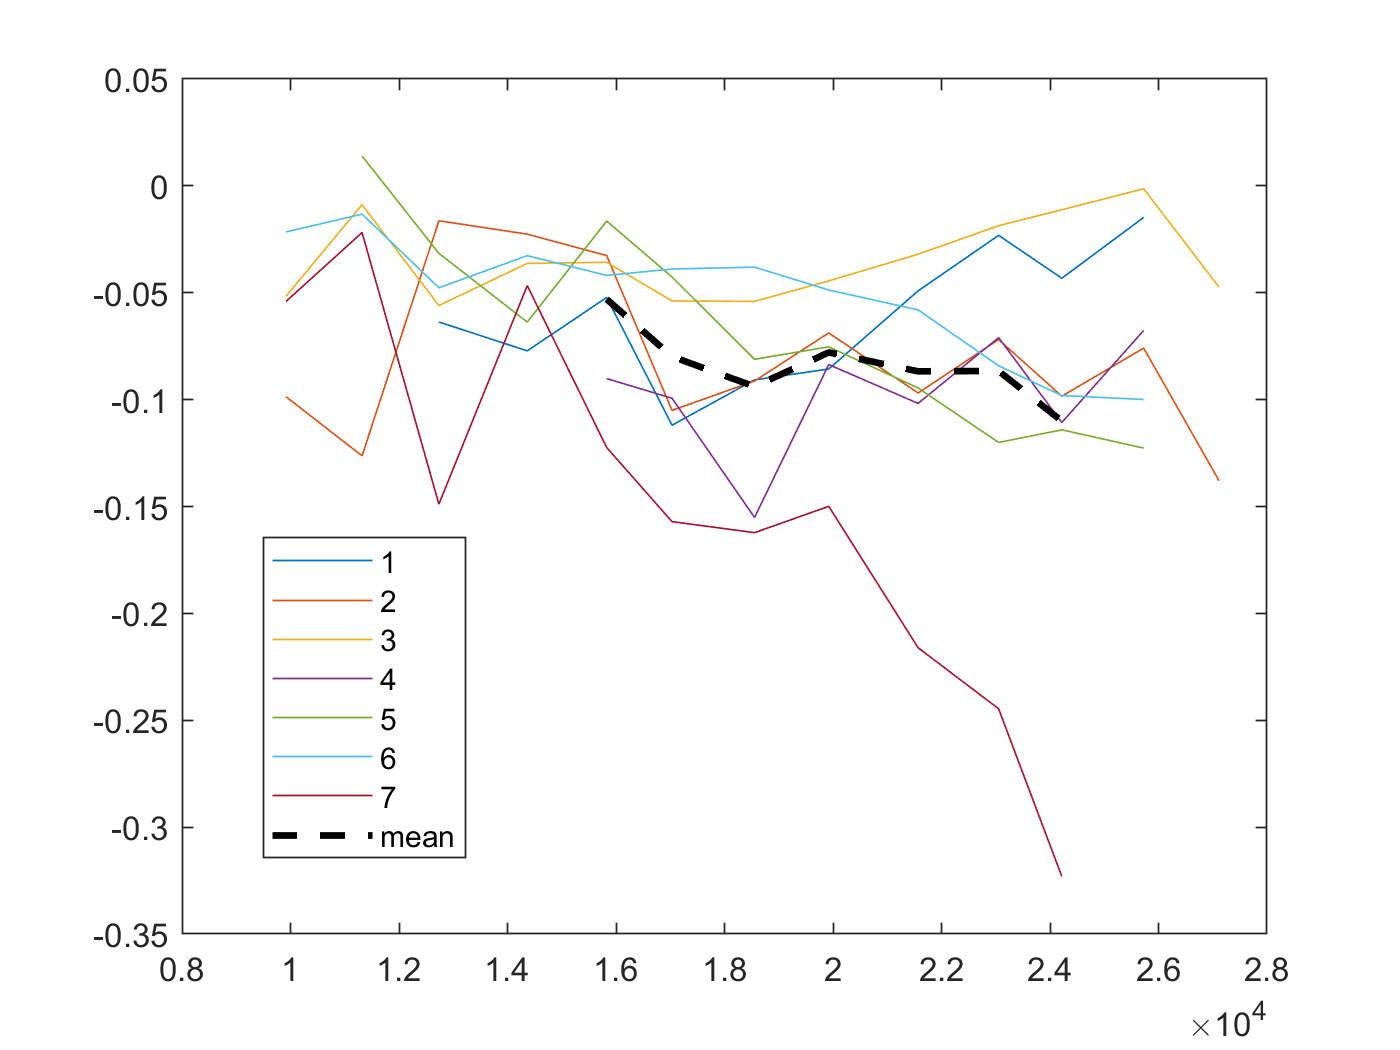
\includegraphics[width=.7\textwidth]{Figures/rlredc50.png}
	\caption{RL phase re OHC-DC at seven positions with arithmetic mean. 50 dB SPL.}
	\label{rlredc50}
\end{figure}

\begin{figure}
	\centering
	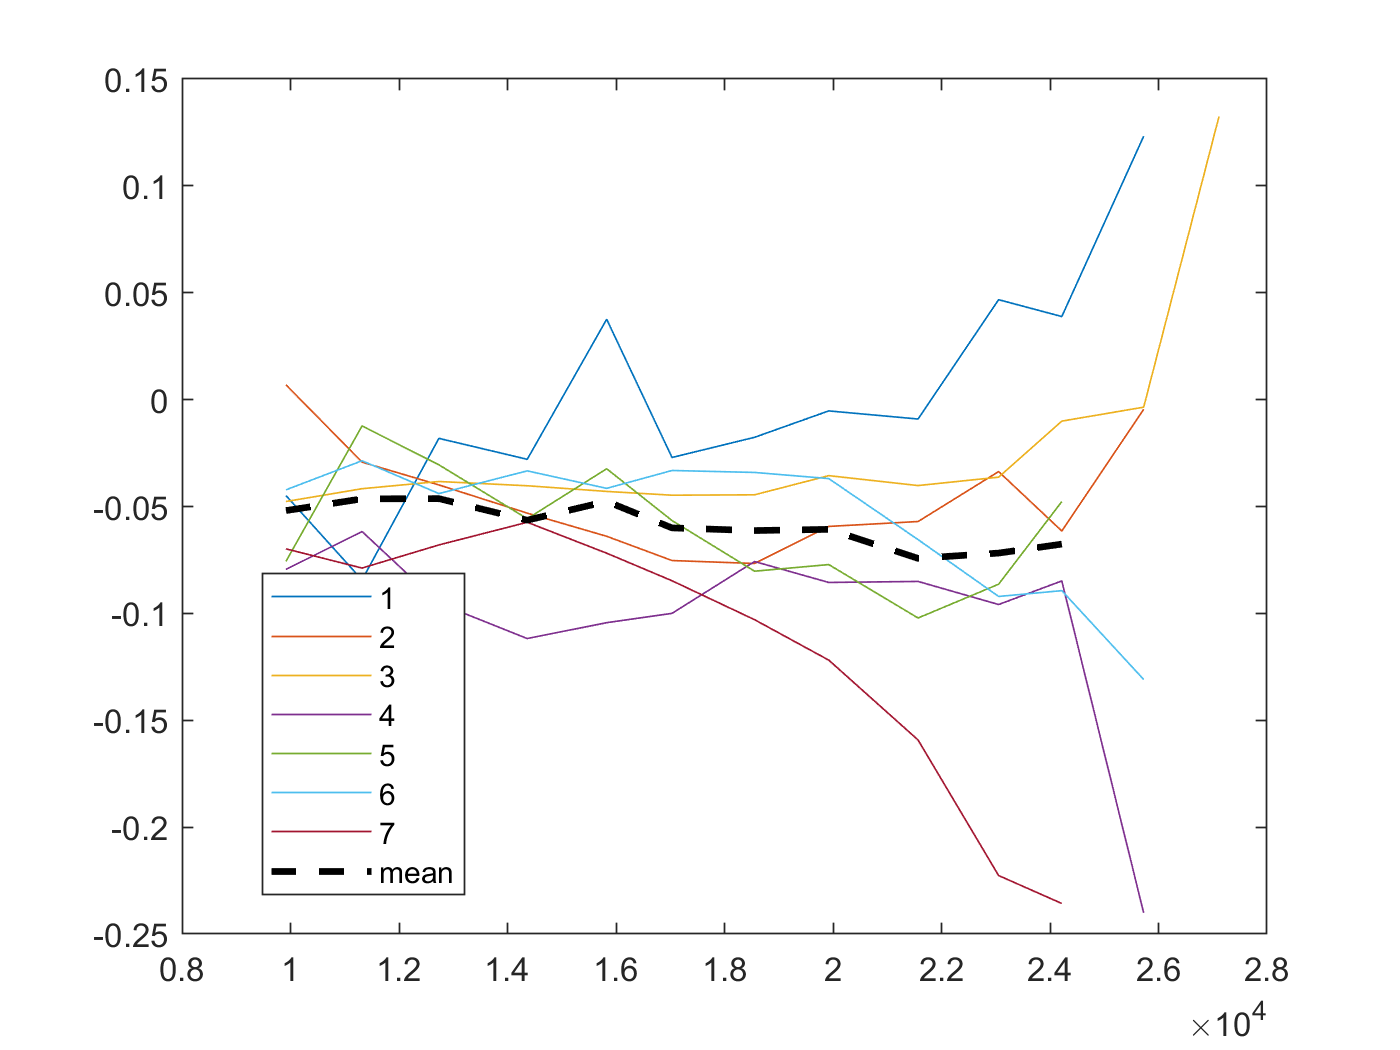
\includegraphics[width=.7\textwidth]{Figures/rlredc65.png}
	\caption{RL phase re OHC-DC at seven positions with arithmetic mean. 65 dB SPL.}
	\label{rlredc65}
\end{figure}

\begin{figure}
	\centering
	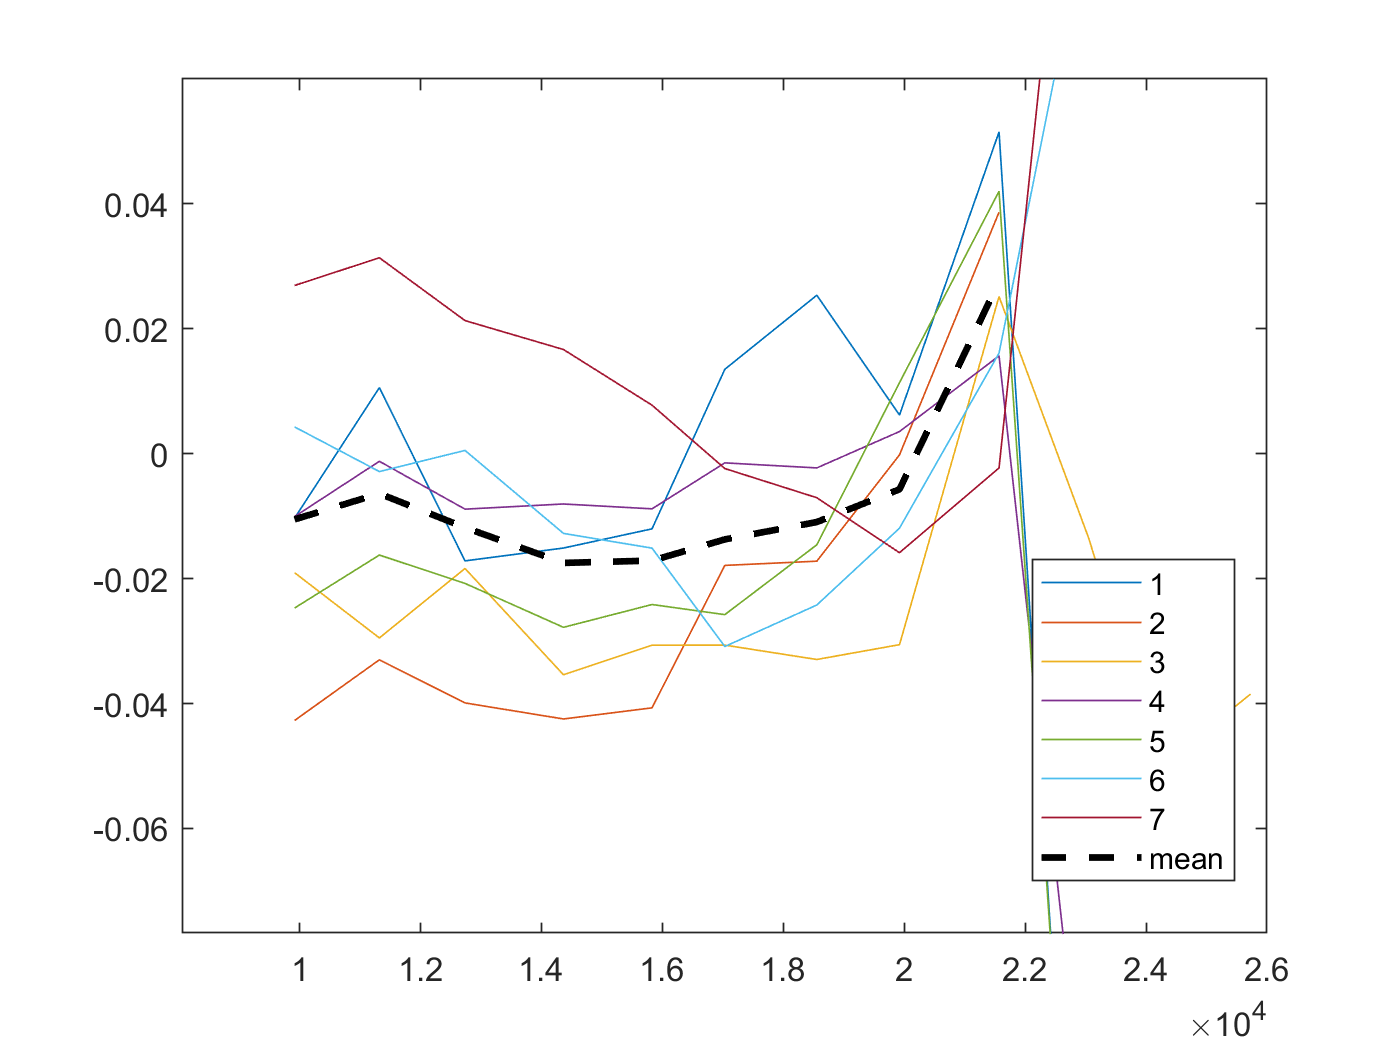
\includegraphics[width=.7\textwidth]{Figures/rlredc80.png}
	\caption{RL phase re OHC-DC at seven positions with arithmetic mean. 80 dB SPL.}
	\label{rlredc80}
\end{figure}

\par{We see that at lower SPLs, OHC-DC leads RL at almost every position, on average by ~20 degrees (although at some positions we see this lead decrease at 65 dB SPL. At 80 dB SPL the two seem to be more-or-less in phase. That is, at our measurement angle we see an OHC-DC lead re RL that decreases as SPL increases.}
\par{Also at 80 dB SPL at high frequencies, we see strange behavior where the OHC-DC re BM lead becomes a lag, very quickly flying upwards in phase. This difference occurs a near the BF, where Dewey also sees a reduction in this lead at 70 dB SPL. We see this at some positions at 65 dB, and at all positions at 80 dB SPL.}
\subsection{Preliminary theories for why we see these motion patterns}
\par{We see far less of a phase difference than Dewey does, but two aspects of our measurement angle are different –- 1) we have a large longitudinal component that he does not likely have; 2) he measures with a large radial component, with a measurement angle parallel to the length of the OHC. This is likely to show the effects of electromotility more directly, but it obscures transverse-longitudinal motion components.}
\par{In our B-Scans, the OHCs appear to lie at a 30 degree angle to the transverse direction, so this OHC-length-axis component has a projection of 0.5 magnitude onto the transverse axis. Our angle has ~0.6 component in the transverse direction, leading to ~0.25 of this component being represented onto our axis of measurement. Then, who knows what’s bigger than what! This is all to say that there is a LOT obscuring this axis of motion.}

\par{Our OHC-DC region measurements at 80 dB SPL are in line with our reconstructions, and at lower SPL seem to imply that transverse motion is more dominant at 50 and 65 dB than at 80 dB. This is what one would expect due to compressive nonlinearity, where the transverse motion caused by the OHCs does scales up \textit{less} as SPL increases.}

\par{As for RL, we see at high SPL they move almost the same as OHC-DC and thereby could have a similar reconstruction. This could mean that the gross transverse motion of the OCC would be contributing to OHC transverse motion more than electromotility, which is expected. However, at lower SPLs we see that RL moves very similarly to OHC-DC with only a ~constant phase difference. This indicates that the transverse component of motion is impacted more by electromotility at lower SPLs. Again, this is what one would expect due to compressive nonlinearity.}

\section{A Simple Model for Transverse-Radial OHC Motion}
\subsection{Outline of the model}
\par{My goal is to reconcile different measurements from the groups of Dewey, Ren and Olson of the ``OHC region" motion. I have measured 1-D OHC-DC and RL motion with longitudinal and transverse components, and reconstructed transverse-longitudinal motion of the OHC-DC region in the gerbil base. Ren has measured 1-D purely transverse motion of the RL, and also 1-D motion of the RL with transverse and longitudinal components in gerbil base and mouse apex. Strimbu and Fallah have measured 1-D motion with components in all three dimensions in both gerbil and guinea pig. Dewey has measured radial-transverse motion along the OHC length axis in the mouse apex.}
\par{With this wealth of data, from different preps, locations and species, it is difficult to integrate this information into a single model, especially at multiple SPLs. However, assuming certain similarities, we do actually have enough information to guess at radial, transverse and longitudinal components. My goal is to draw hypotheses from each of these experiments, and use them to create a ``reasonable" guess of the motion at the RL and OHC-DC under an extremely simple model, and see if I can produce similar results to what is seen in all of these experiments via projection. Starting with a purely radial-transverse model, these are my hypotheses:}
\begin{enumerate}
	\item{Radial-transverse OHC motion is a combination of two components -- a \textit{gross transverse motion} wherein the entire OCC moves as one, and a \textit{piezoelectric motion} wherein the OHC expands and compresses along the axis parallel to its length.}
	\item{Gross transverse motion is equal to BM motion near the OHC-DC region.}
	\item{The RL and OHC-DC piezoelectric motions are out of phase by 0.5 cycles at all frequencies, and equal in magnitude.}
	\item{Transverse RL motion precisely as seen in Ren's data (ARO 2022).}
\end{enumerate}
\par{A cartoon of this gross-piezoelectric decomposition is shown in Fig \ref{grosspiezo}. The reader may be either happy or unhappy at the fact that this introduces a \textit{fourth} axis to the physiological problem -- that which is parallel to the length of the OHC. It is along this axis that the OHC expands and compresses, so this is a necessary focus for our model. Moreover, a ``gross-piezoelectric" decomposition offers more physiological insight into the motion than an orthogonal radial-transverse decomposition, in my opinion.}

\begin{figure}
	\centering
	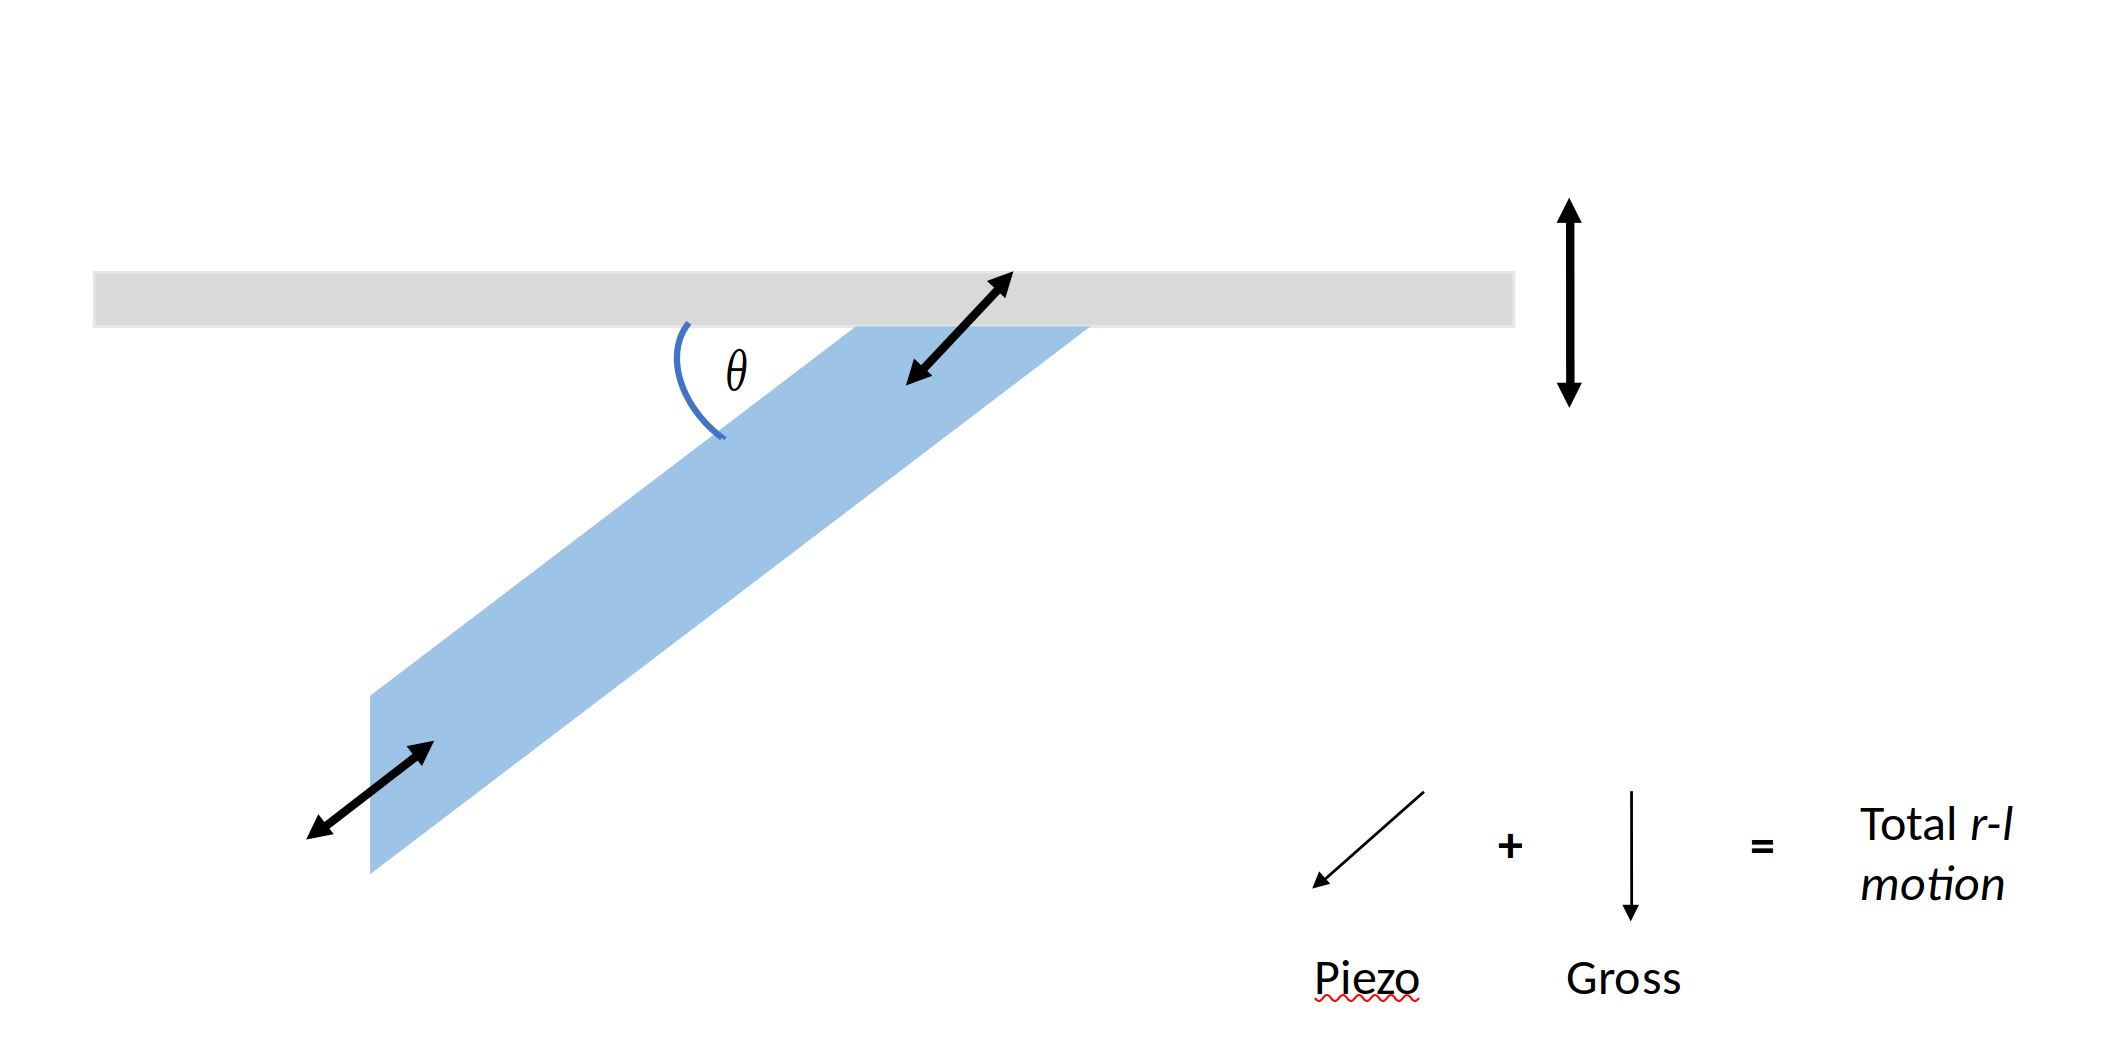
\includegraphics[width=0.7\textwidth]{Figures/grosspiezo.png}
	\caption{A cartoon of the BM (gray) and an OHC (blue). The whole structure moves with a gross transverse component equal to BM motion. The OHCs expand and contract piezoelectrically along their own axis, with RL 0.5 cycles out of phase with OHC-DC.}
	\label{grosspiezo}
\end{figure}

\subsection{Mathematics of the model}
\par{The data fed into the model is that of Ren -- purely transverse RL motion $R_t$, and purely transverse BM motion near the RL, $B$. We say the BM motion near the OHC-DC region is our gross transverse motion, and our data shows that BM motion near OHC-DC is aboout 1.5 times as large as BM motion near the RL. We say the gross motion is $G = 1.5B$. Recall that all of these quantities are complex phasors as functions of frequency, containing magnitudes \textit{and} phases.}
\par{We say the RL motion along the piezoelectric axis is $R_p$. If the BM and OHC make an angle $\theta = 30^{\text{o}}$, then the total RL motion along the transverse axis is the sum of the gross motion and the piezo motion projected onto the transverse axis:
	\begin{equation}
		R_t = G + R_p \sin{\theta}.
	\end{equation}
We feed in Ren's $R_t$, so this gives us the piezoelectric motion of RL.}
\par{Our hypothesis is that OHC-DC piezoelectric motion is equal in magnitude to RL piezoelectric motion and out of phase by 0.5 cycles, or $\pi$ radians. This gives $D_p = -R_p$, as $e^{j\pi} = -1$. In terms of the Ren data we have, we can write:
	\begin{align}
		G &= 1.5B, \\
		R_p &= \frac{G - R_t}{\sin\theta}, \\
		D_p &= -R_p, \\
		D_t &= G + D_p\sin\theta.
	\end{align}
}
\par{Finally, we consider data as measured along the OHC's axis. This is not purely piezoelectric motion but also contains the gross component projected along this axis. These are given by
	\begin{align}
		R_o &= R_p + G\sin\theta, \\
		D_o &= D_p + G\sin\theta.
	\end{align}
This gives us the RL and OHC-DC region as measured purely transversely, as well as measured along the OHC axis. Consideration of other measurement axes just requires the projections of these quantities onto different axes, and might be important for future studies.}
\subsection{Model results}
\par{Figs \ref{grosspiezot} and \ref{grosspiezoo} show the OHC motion derived from this model as measured along the transverse and OHC axis respectively, at 20, 40, 60 and 80 dB SPL. Taking the difference of OHC-DC phase and RL phase along the OHC axis, we compare our OHC-DC re RL phase to Dewey's and see a nice agreement in Fig \ref{reconstructeddewey}.}

\begin{figure}
	\centering
	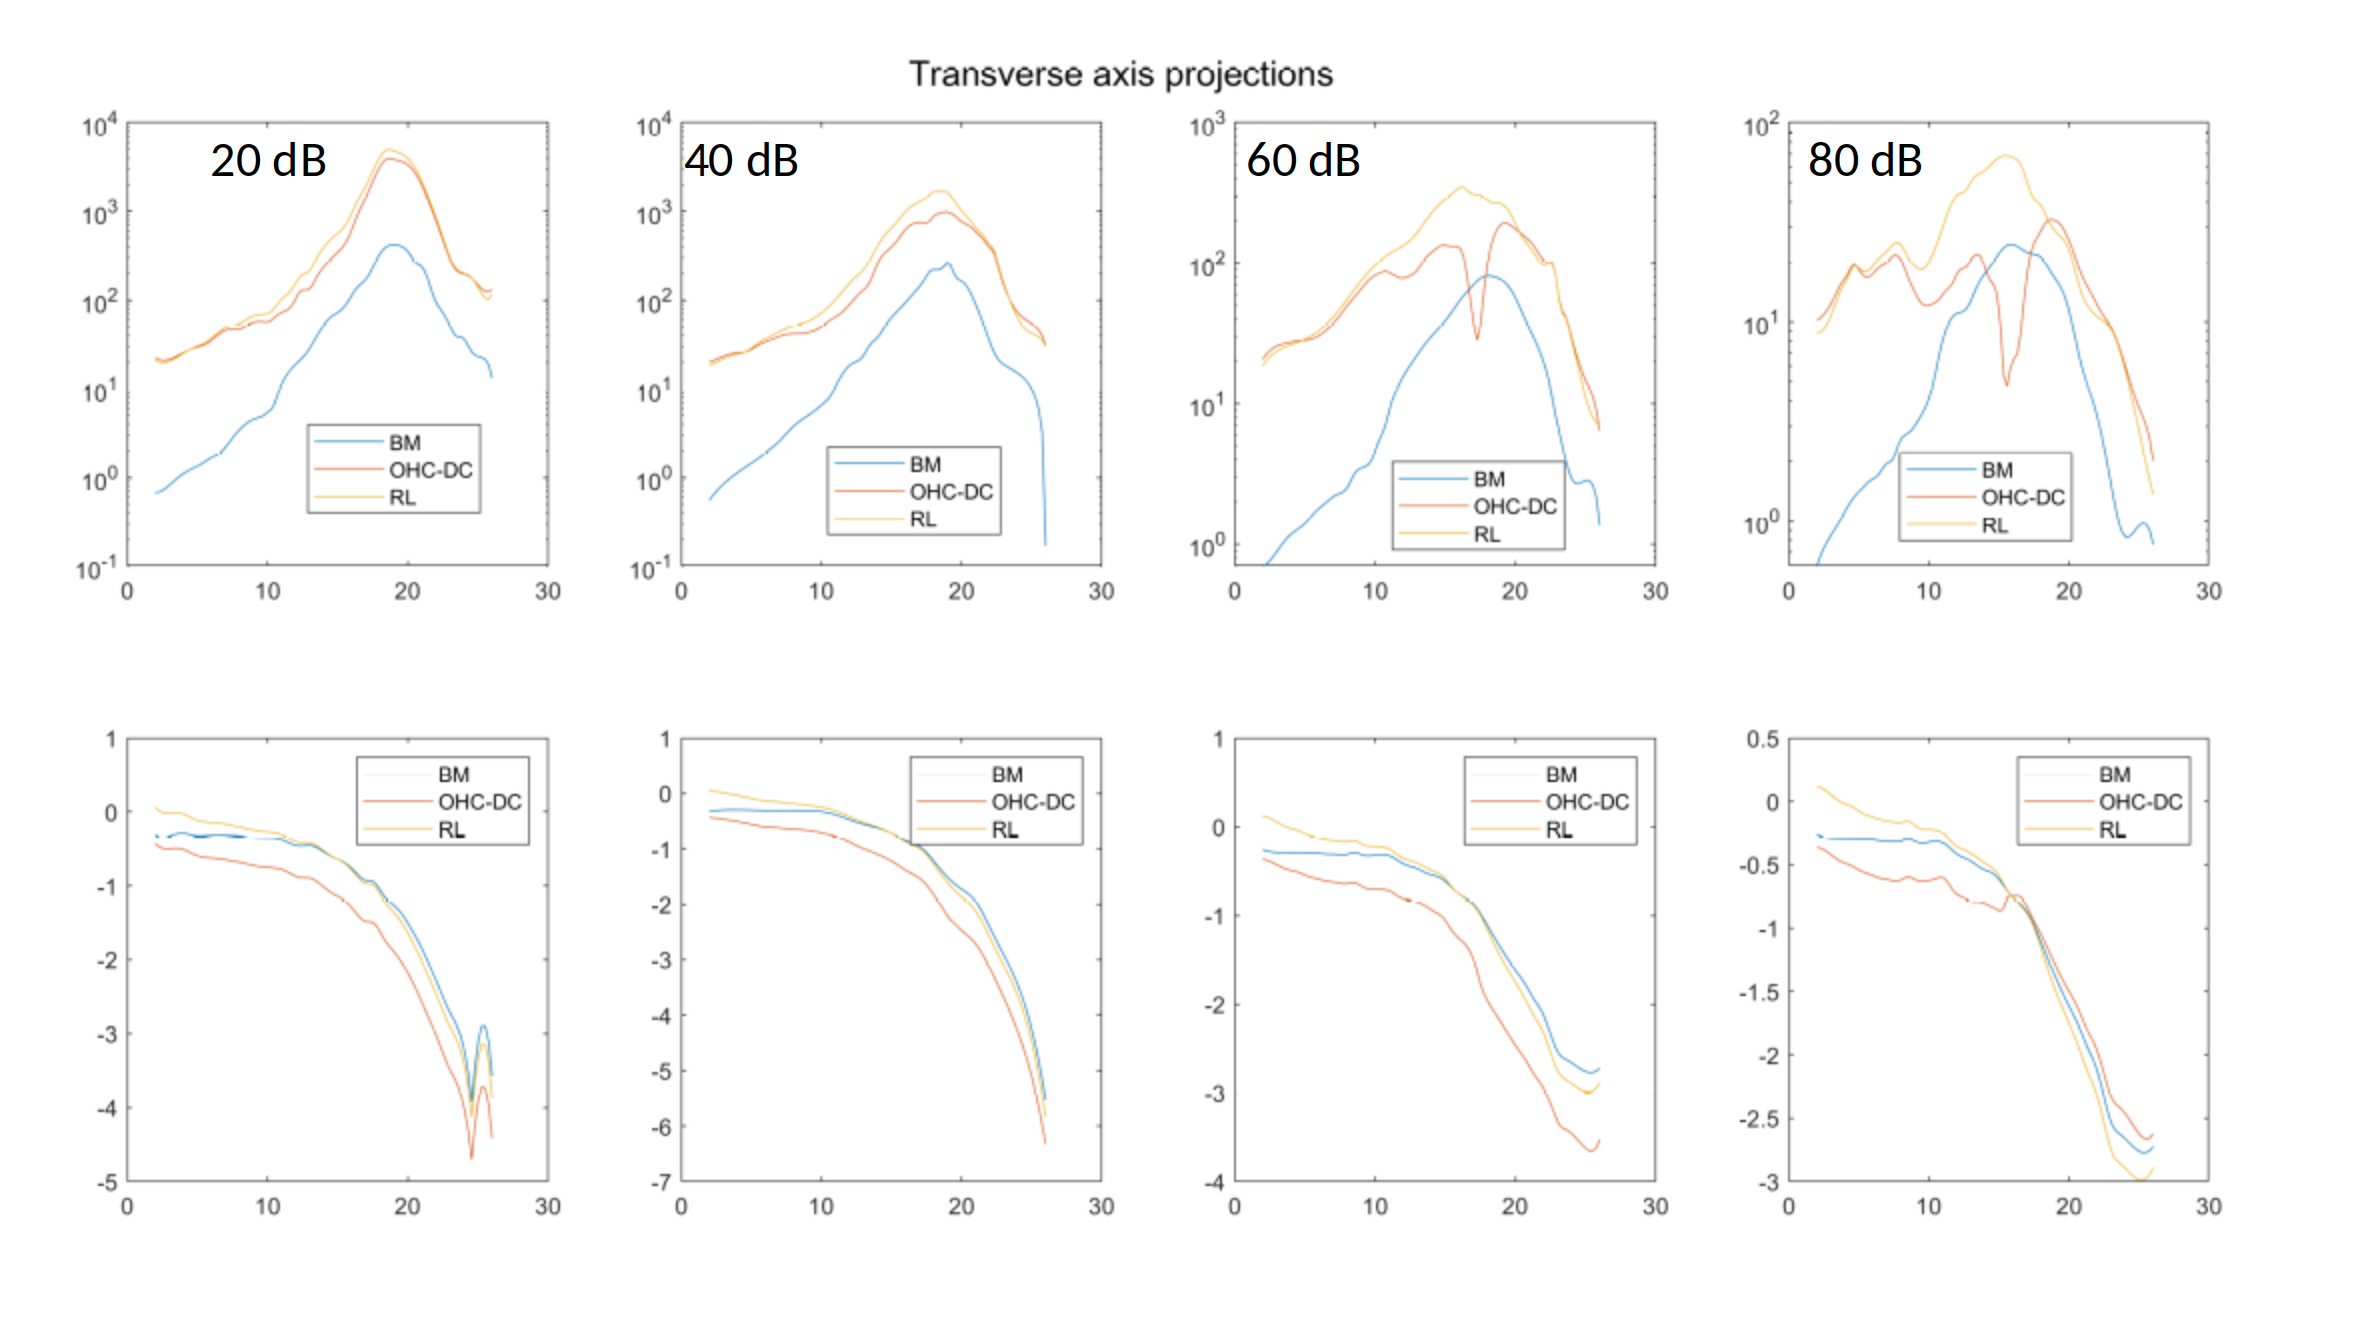
\includegraphics[width=\textwidth]{Figures/grosspiezot.png}
	\caption{Modeled OHC-DC and RL gain re stapes as measured along the transverse axis at 20, 40, 60 and 80 dB SPL.}
	\label{grosspiezot}
\end{figure}

\begin{figure}
	\centering
	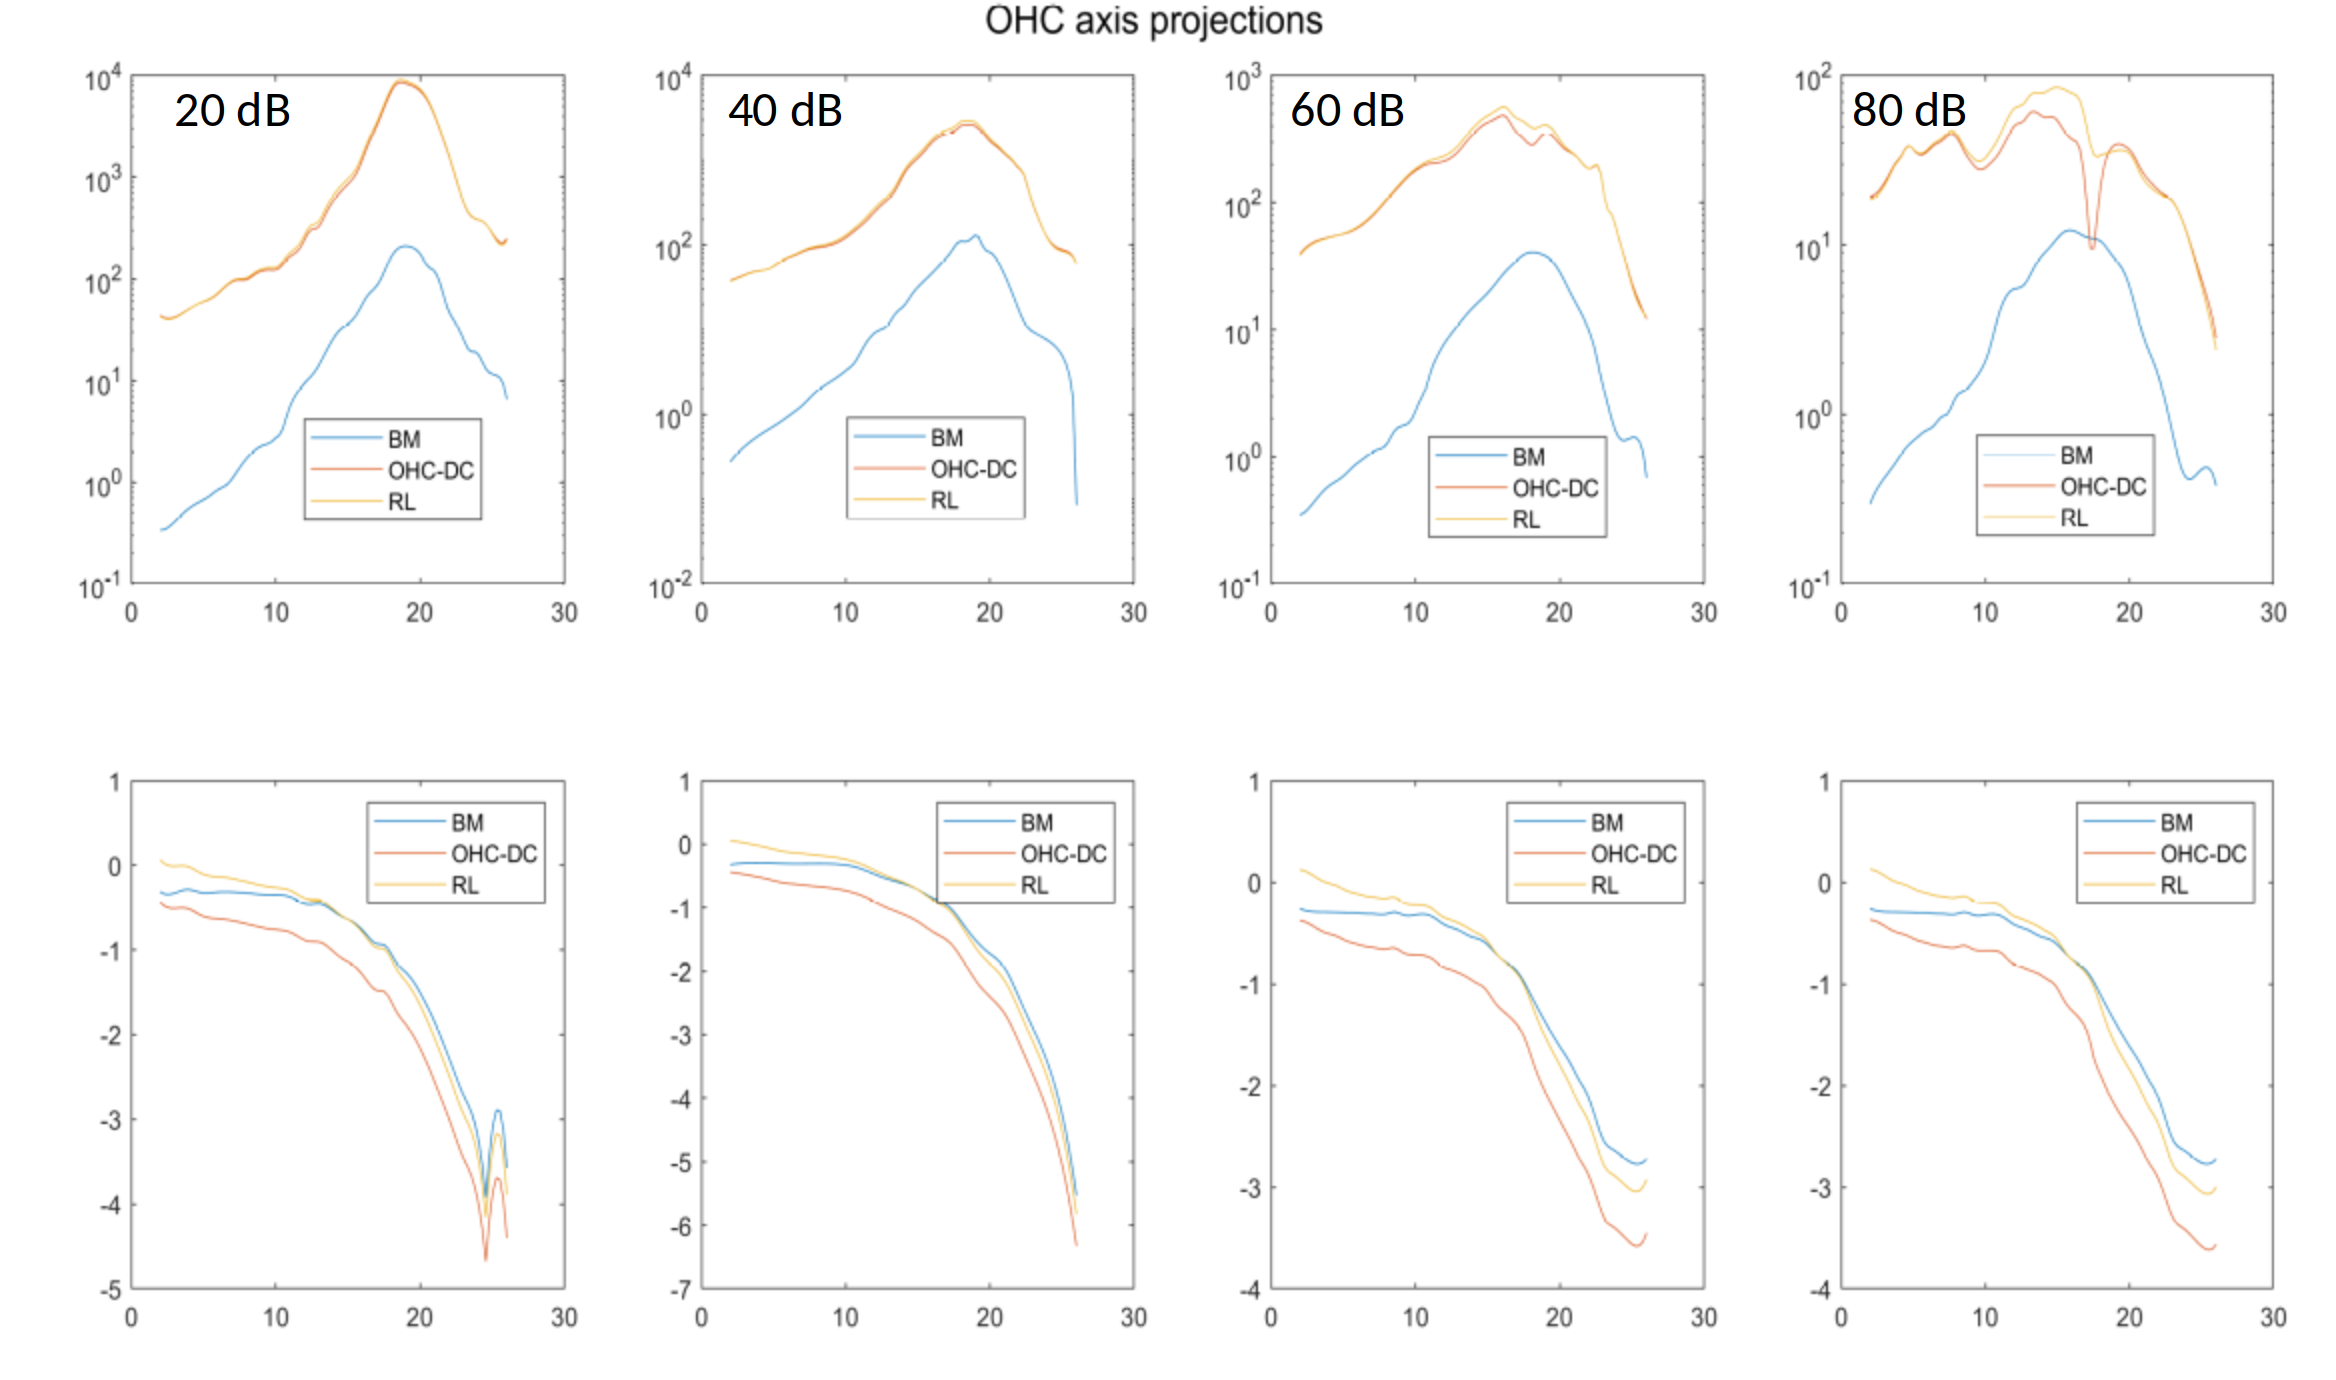
\includegraphics[width=\textwidth]{Figures/grosspiezoo.png}
	\caption{Modeled OHC-DC and RL gain re stapes as measured along the OHC axis at 20, 40, 60 and 80 dB SPL.}
	\label{grosspiezoo}
\end{figure}

\begin{figure}
	\centering
	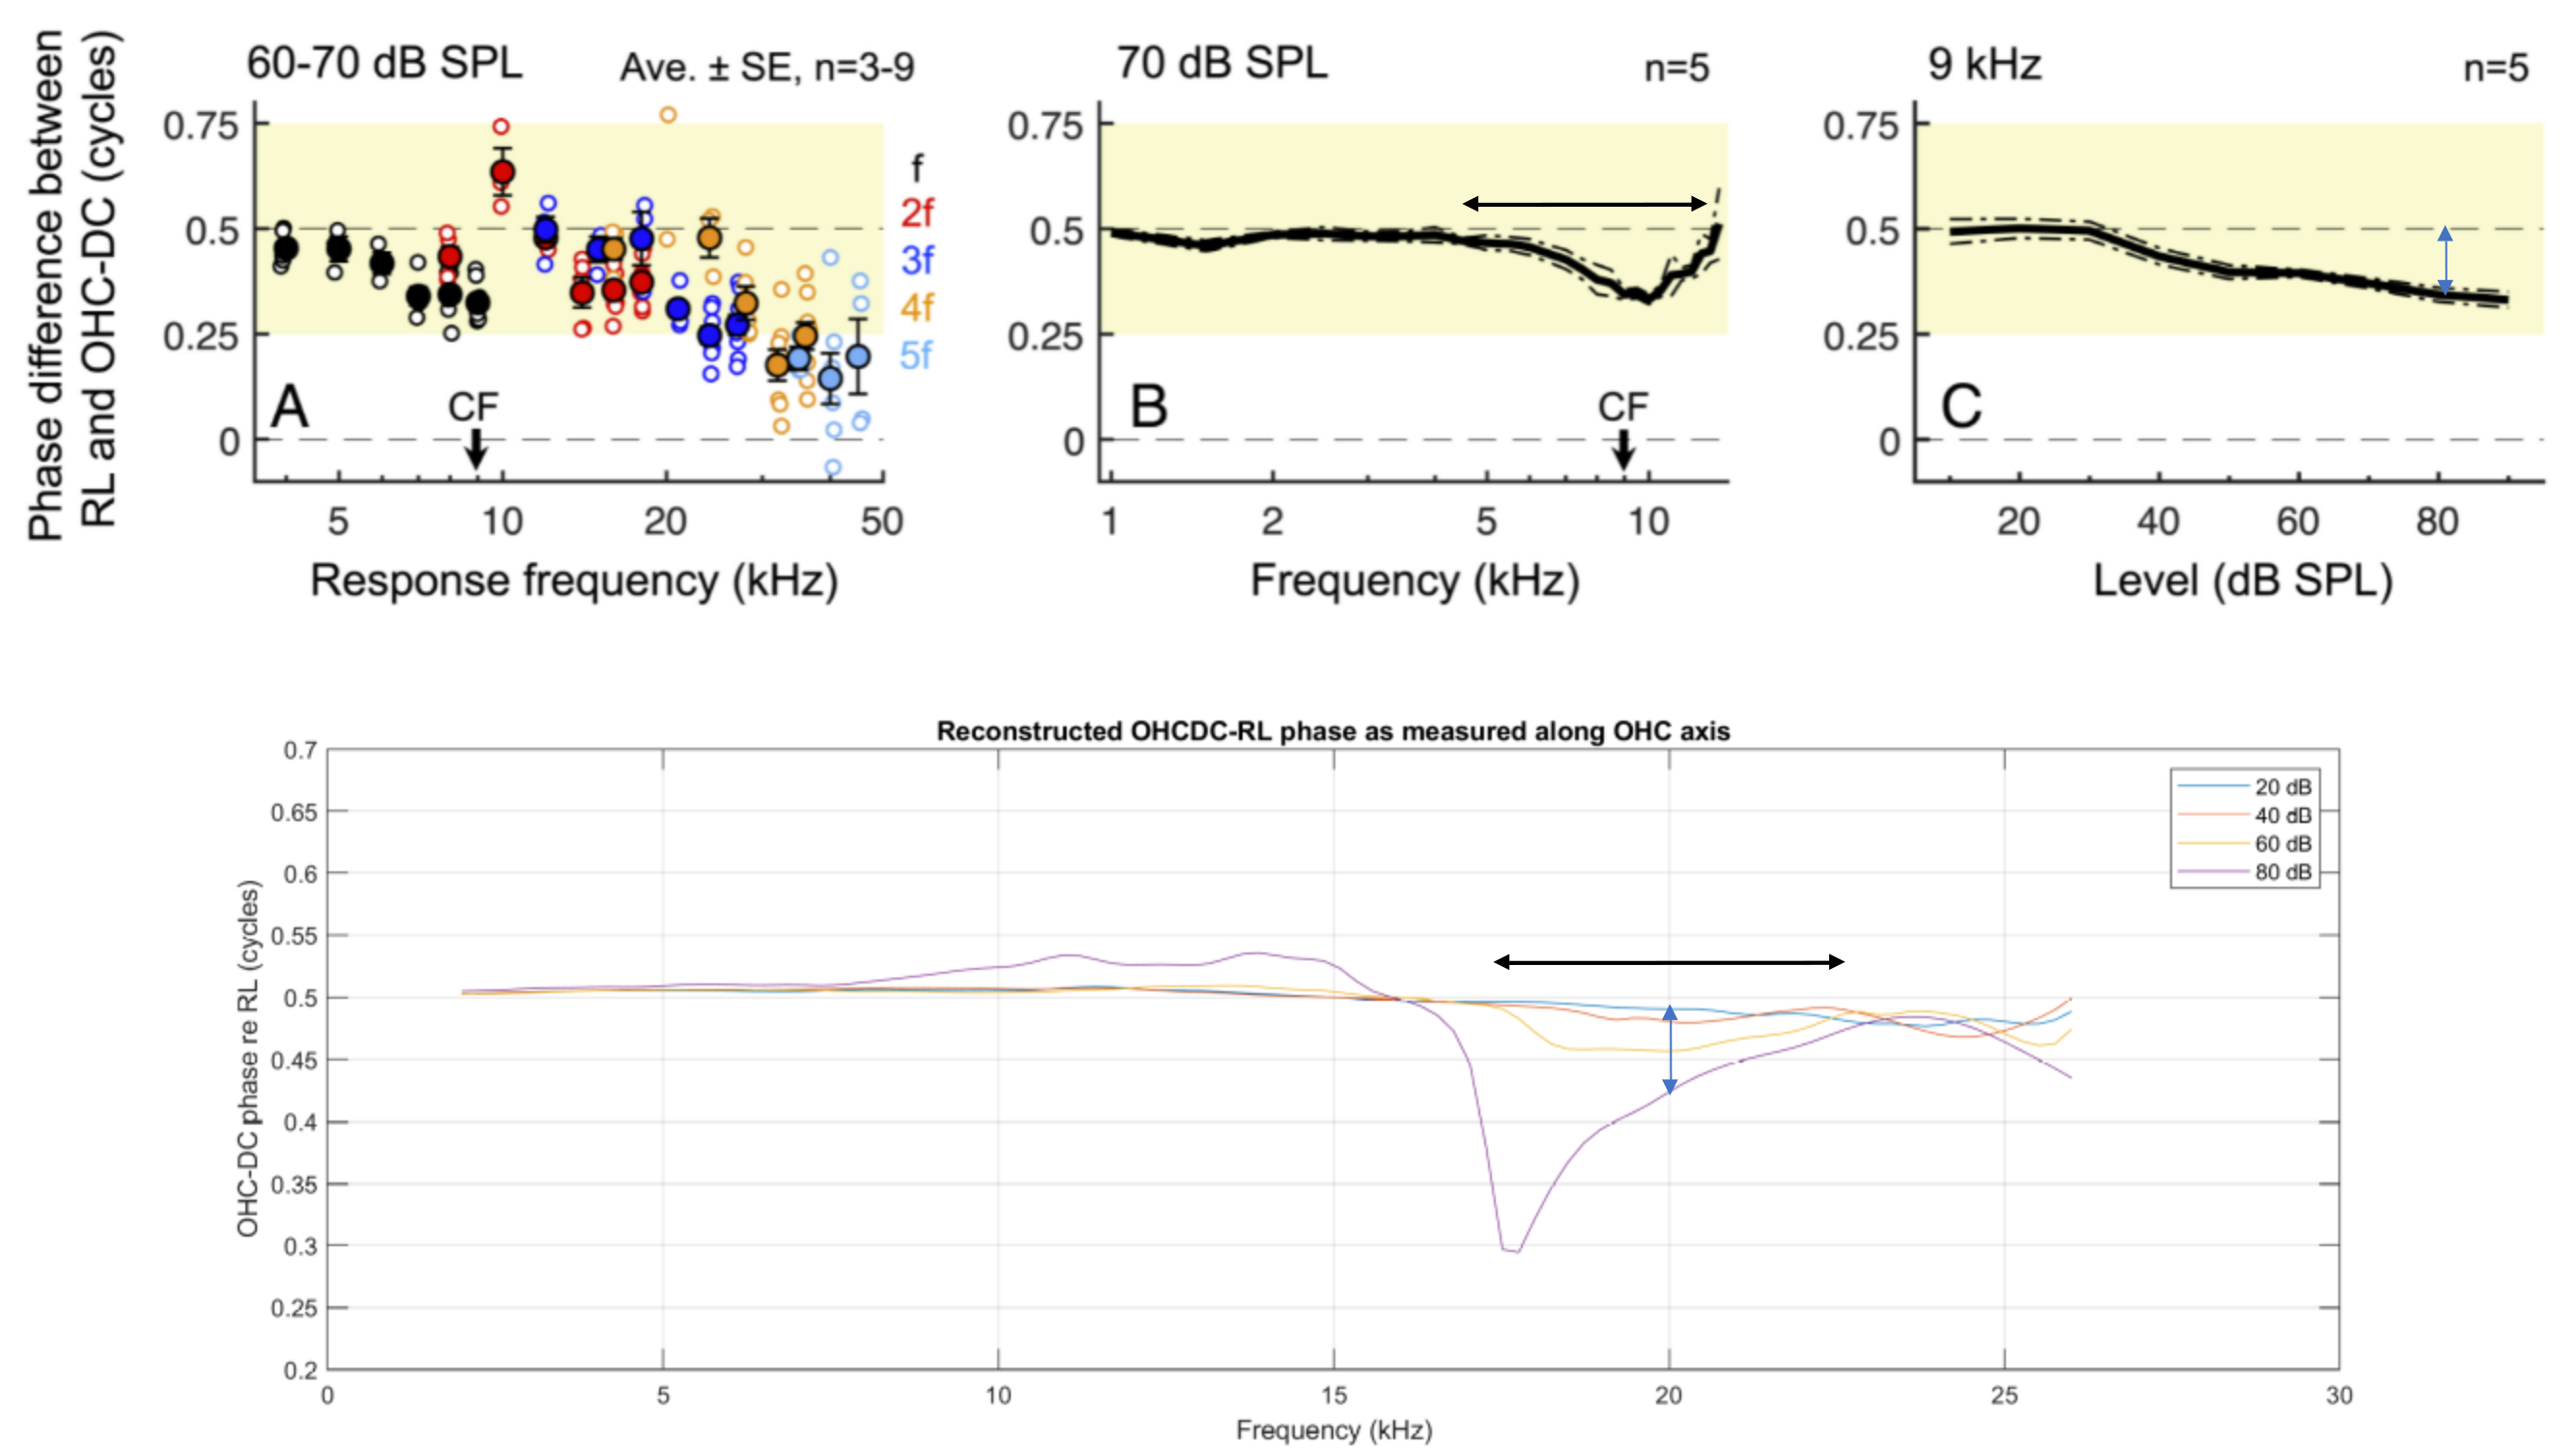
\includegraphics[width=\textwidth]{Figures/reconstructeddewey.png}
	\caption{Panels above are from Dewey, showing a 0.5 cycle OHC-DC lead re RL at 70 dB SPL at low frequencies, which dips near the BF. Also shown is SPL dependence of the OHC-DC re RL lead at BF, which diminishes at high SPLs. Below is our reconstruction of OHC-DC phase re RL as measured along the OHC axis. We see also that at low frequencies the lead is 0.5 cycles and dips near BF. We also see that the lead diminishes more as SPL increases.} 
	\label{reconstructeddewey}
\end{figure}

\par{Our data seem to show that under basic assumptions, the Dewey and Ren data are consistent with one another. Of course, the OHC axis was not Dewey's measurement axis. Further work may observe how this model shows phase differences along other axes.}
\par{Our model adds a layer of interpretation onto the Dewey data that is otherwise obscured -- why is there a dip in the OHC-DC lead around the BF, and why does this dip become more severe at higher SPL? Our model suggests that this is due to a takeover of gross motion, i.e. the large BM motion that dominates in the high-SPL and BF regimes.}
\section{Conclusions and Future Work}
\par{Our reconstructions and longitudinal studies have shown that transverse motion dominates longitudinal motion (a) near BF, and (b) at high SPLs. We have shown that the deviation from the 0.5 cycle difference expected, as seen by Dewey, can reasonably be due to dominating transverse motion near CF and at high SPLs (now in the radial-transverse plane). We have shown that Dewey’s and Ren’s measurements are totally consistent and the interpretation of ``gross-piezoelectric” decomposition nicely generates the character of Dewey’s data from Ren’s. Our data is quite similar to Ren's when reconstructed into transverse and longitudinal components at 80 dB SPL.}
\par{However, the phase difference we measure between OHC-DC and RL is very small compared to Dewey's, even at low SPL, and deserves an explanation. This could be due to geometrical factors induced by our large longitudinal angle, or due to our mislabeling of OHC-DC and RL. This potential for mislabeling could also be present in Ren's data.}
\par{In future, I would like to synthesize these data with our longitudinal-transverse measurements using a hopefully similar simple model. I would like to analyze the many studies done in guinea pig and gerbil from our lab, taken at various angles, to analyze the character of these measurements in this new light. I would also like to perform transverse-longitudinal reconstructions of RL motion and OHC-DC motion at lower SPLs.}
\end{document}
